\documentclass[pdflatex,11pt]{aghdpl}
% \documentclass{aghdpl}               % przy kompilacji programem latex
% \documentclass[pdflatex,en]{aghdpl}  % praca w jêzyku angielskim
\usepackage[polish]{babel}
\usepackage{polski}
\usepackage[utf8]{inputenc}

% dodatkowe pakiety
\usepackage{enumerate}
\usepackage{hyperref}

% Listings ------------------------------------------------------------
\usepackage{listings}
% Scala listings
% "define" Scala
\lstdefinelanguage{scala}{
  morekeywords={abstract,case,catch,class,def,%
    do,else,extends,false,final,finally,%
    for,if,implicit,import,match,mixin,%
    new,null,object,override,package,%
    private,protected,requires,return,sealed,%
    super,this,throw,trait,true,try,%
    type,val,var,while,with,yield},
  otherkeywords={=>,<-,<\%,<:,>:,\#,@},
  sensitive=true,
  morecomment=[l]{//},
  morecomment=[n]{/*}{*/},
  morestring=[b]",
  morestring=[b]',
  morestring=[b]"""
}

% IntelliJ Colors for listings
\usepackage{color}
\definecolor{dkgreen}{rgb}{0,0.6,0}
\definecolor{gray}{rgb}{0.5,0.5,0.5}
\definecolor{mauve}{rgb}{0.58,0,0.82}
 
% Default settings for code listings
\lstset{
  frame=tb,
  language=Scala,
  aboveskip=3mm,
  belowskip=3mm,
  showstringspaces=false,
  columns=flexible,
  basicstyle={\small\ttfamily},
  numbers=none,
  numberstyle=\tiny\color{gray},
  keywordstyle=\color{blue},
  commentstyle=\color{gray},
  stringstyle=\color{dkgreen},
  frame=single,
  breaklines=true,
  breakatwhitespace=true
  tabsize=3
}

\lstloadlanguages{TeX}

%---------------------------------------------------------------------------

\author{Konrad Malawski}
\shortauthor{K. Malawski}

\titlePL{ProtoDoc\\Implementacja odpowiednika narzędzia JavaDoc dla jęzka definicji interfejsów Google~Protocol~Buffers}
\titleEN{ProtoDoc\\Development of a JavaDoc tool equivalent for the Google Protocol Buffers Interface~Description~Language}

\shorttitlePL{ProtoDoc - impl. odpowiednika JavaDoc dla Google~Protocol~Buffers} 
\shorttitleEN{ProtoDoc - impl. of JavaDoc like tool for Google~Protocol~Buffers}

\thesistypePL{Praca Dyplomowa Inżynierska}
\thesistypeEN{Bachelor of Science Thesis}

\supervisorPL{dr inż. Jacek Piwowarczyk}
\supervisorEN{Jacek Piwowarczyk Ph.D}

\date{2012}

\departmentPL{Katedra Automatyki}
\departmentEN{Department of Automatics}

\facultyPL{Wydział Elektrotechniki, Automatyki, Informatyki i Elektroniki}
\facultyEN{Faculty of Electrical Engineering, Automatics, Computer Science and Electronics}

\acknowledgements{} % TODO podziękowania

\setlength{\cftsecnumwidth}{10mm}

%---------------------------------------------------------------------------

\begin{document}

\titlepages

\tableofcontents
\clearpage

%---------------------------------------------------------------------------------------------------------------------------------------------------------------------------
\chapter{Wprowadzenie}
\label{cha:wprowadzenie}

Poniższy rozdział ma za cel przedstawienie czytelnikowi dziedziny oraz problemu jaki rozwiązuje zaimplementowany 
w ramach tej pracy inżynierskiej program - \textit{ProtoDoc}. Następnie zostaną przedstawione rozdziały pracy oraz jakie 
tematy dany rozdział porusza.

\section{Przedstawienie dziedziny zagadnienia}

Google Protocol Buffers są zespołem narzędzi i binarnego protokołu służącymi do transportu danych w możliwie najefektywniejszy sposób.
Można o nich myśleć w kategorii następcy takich formatów danych jak XML lub ostatnio popularny JSON. Główną przyczyną dlaczego Protocol Buffers, 
dalej zwanymi ProtoBuf, zaczynają powoli wypierać zastosowanie wcześniej wspomnianych formatów reprezentacji danych jest fakt wynikający bezpośrednio
z części ,,binarny'' w opisie ProtoBuf -- wiadomości kodowane przy pomocy tego narzędzia, mogą być znacznie efektywniej kompresowane oraz szybciej 
rekonstruowane. W przypadku systemów ,,High Velocity'' gdzie opóźnienia rzędu milisekund już są znaczące okazuje się, że nie ma już od dawna miejsca
dla uznawanych dotychczas przez branżę standardów komunikacji, takich jak na przykład SOAP, parsowanie którego wiadomości z racji formatu danych, zwyczajnie
nie jest w stanie sprostać wymaganiom wydajnościowym tych systemów. Jednym z przykładów największych instalacji ProtoBuf jest oczywiście samo Google, 
stosujące je w ramach komunikacji między większością swoich aplikacji. Protocol Buffers nie są same w ruchu wielkich firm ku binarnym protokołom - 
jako przykład może posłużyć \href{http://thrift.apache.org/}{Apache Thrift} \cite{Thrift}, będący odpowiednikiem ProtoBuf,
uwolnionego jako open source spod skrzydła Facebook. 

Zasada działania tych protokołów jest prosta, oraz w pewien sposób zbliżona do tego co świat enterprise zna od lat, pod formą WSDL, to znaczy ,,kontraktów''
między dostawcą serwisu oraz jego klientami. W Protocol Buffers taki kontrakt spisuje się przy pomocy specjalnego IDL (\textit{Interface Description Language} 
- ang. Język opisu interfejsu) o tej samej nazwie. Język ten jest przedmiotem niniejszej pracy inżynierskiej. Definiowane przy jego pomocy typy wiadomości
są następnie wykorzystywane przez kompilator \textit{protoc}, celem generowania ,,potrafiących się przeczytać ze strumienia bajtów'' klas, w dowolnym języku
programowania. Pozwala to na automatyczne generowanie web serwisów, analogicznie jak miało to miejsce w przypadku generowania kodu z WSDL za czasów SOAP.

Miejscem w którym \textit{ProtoDoc}, aplikacja powstała w ramach tej pracy inżynierskiej, znajduje swoją niszę, jest dokumentacja wiadomości Protocol Buffers.
Niestety okazuje się, iż dokumentacja wiadomości Protocol Buffers staje się dużym problemem w korporacjach gdzie mamy do czynienia setkami wiadomości, które
zostały pierwotnie stworzone wiele lat temu. Niestety nie istnieją obecnie narzędzia generujące dokumentację na podstawie kodu ProtoBuf. Pomogłoby
to rozproszonym dużym zespołom uniknąć nieporozumień dotyczących poprawnego wykorzystywania wiadomości. Narzędziem które może ten stan rzeczy zmienić,
jest \textit{ProtoDoc}.


%---------------------------------------------------------------------------
\section{Cel pracy}
\label{sec:celePracy}

Celem projektu jest implementacja narzędzia generującego dokumentację na podstawie plików 
*.proto zawierających zapisane przy pomocy ,,języka definicji interfejsów'' (tzw. \textit{Interface Description Language}, w skrócie \textit{IDL}) - Google Protocol Buffers. 


Potrzebę implementacji takiego narzędzia motywuję doświadczeniem w pracy z Protocol Buffers, gdy mamy do czynienia z dużą ilością plików *.proto (setki). 
Brak automatycznie generowanej dokumentacji tak dużego zbioru wiadomości znacznie utrudniał zapoznanie się z systemem oraz przystąpienie do sprawnej pracy z nim.
Gdyby taka, zawsze aktualna, dokumentacja była dostępna w firmowym intranecie na przykład, komunikacja między zespołami o wiadomościach byłaby znacznie prostsza - 
możliwe byłoby wówczas przesłanie sobie między programistami linku do właściwej wiadomości ,,to tej wiadomości szukasz'', włącznie z upewnieniem się, że na pewno
wskazana wiadomość nie jest przestarzała - zawierałaby wówczas odnośnik do wiadomości którą obecnie powinno się stosować.


Proces generowania dokumentacji jest analogiczny do znanego z świata Javy narzędzia JavaDoc \cite{JavaDoc} - stąd zainspirowana JavaDociem nazwa tego projektu. 
Sam proces generowania dokumentacji polega na dostarczeniu narzędziu plików *.proto, które następnie są parsowane oraz na podstawie tego procesu, 
generowana jest strona www zawierające wszystkie zebrane informacje, włącznie z komentarzami oraz dodatkowymi informacjami 
typu ,,\textit{deprecated}'' (ang. przestarzałe). Jako dodatkowy krok wygenerowana strona mogłaby automatycznie zostać opublikowana w firmowym intranecie.

Cały proces możliwe jest w pełni zintegrować z narzędziami stosowanymi do budowania projektów np. Javowych. W przypadku projektów Javowych, obecnym \textit{de facto}
standardem w wielu firmach stał się Apache Maven \cite{Maven}.
ProtoDoc może zostać użyty razem z Maven aby automatycznie, podczas budowania projektu generować
dokumentację. Możliwe jest uruchomienie tego zadania samodzielnie, lub jako jeden z etapów budowy projektu - dzięki czemu nie konieczne jest pamiętanie oraz ręczne
aktualizowanie dokumentacji - byłaby automatycznie generowana podczas buildu, na przykład na serwerze ciągłej integracji.

\section{Zawartość pracy}
W rozdziale \ref{sec:dostepneNarzedzia} (\textit{Analiza obecnie dostępnych rozwiązań}) zostaną przedstawione obecnie istniejące implementacje parserów Protocol Buffers.
Poddane rozważaniom zostanie opłacalność skorzystania ze wspomnianych rozwiązań open source jako bazy tego projektu.
Ostatecznie jednak przedstawione zostanie ostatecznie wybrane rozwiązanie implementacji parsera zastosowane w tym projekcie - kombinatory parserów języka Scala.

W rozdziale \ref{cha:projekt_systemu} (\textit{Projekt systemu}) omówiona zostanie ogólna architektura aplikacji oraz jej podział na funkcjonalnie niezależne moduły.
Następnie zostaną opisane odpowiedzialności każdego z modułów oraz czytelnik zostanie przeprowadzony przez proces tworzenia hierarchii typów
służącej w całym projekcie to wiernego oraz praktycznego oddania typów oraz pól mogących pojawić się w opisie wiadomości Protocol Buffers.

W kolejnym Rozdziale \ref{sec:zastosowanePodejscie} (\textit{Szczegóły implementacyjne}) zostaną omówione najważniejsze szczegóły implementacyjne każdego z wprowadzonych w poprzednim rozdziale komponentów.
Szczególny nacisk zostanie położony na właściwości języka Scala oraz wybory dokonane w związku z zakresem oraz ewentualną kontunuacj projektu.

Następnie w rozdziale \ref{maven} (\textit{Przykład zastosowania ProtoDoc w realnym projekcie}) przedstawione zostanie jak w praktyce
powinno się korzystać z zaimplementowanego w ramach tego projektu narzędzia. Przedstawiony zostanie również plugin do narzędzia Maven \cite{Maven}
dzięki któremu pełna automatyzacja oraz włączenie ProtoDoc w proces budowania projektu jest bardzo proste.

W przedostatnim rozdziale, tj. \ref{chapter:tdd} (\textit{Rola testów w procesie tworzenia aplikacji}) przedstawiona zostanie metodyka Test Driven Development
(ang. ,,Prowadzenie Projektu Testami'' - tłumaczenie własne), dzięki której każda funkcjonalność przedstawiania w poniższej aplikacji pokryta została 
również automatycznym testem, mogącym potwierdzić poprawne funkcjonowanie aplikacji.

Ostatni rozdział \ref{cha:podsumowanie} (\textit{Podsumowanie}) podsumowuje pracę oraz przedstawiane są w nim możliwości dalszego rozwoju aplikacji.

~\\\*

Jako załączniki do pracy zostały dołączone dwa dodatki:
\begin{itemize}
 \item w Dodatku \ref{cha:appendixA} omawiane są Protocol Buffers -- skąd i dlaczego powstały oraz przedstawia 
       podstawowe zastosowanie ich w praktyce, 
 \item w Dodatku \ref{cha:appendixB} natomiast przedstawiany jest język Scala oraz Parser Combinators. Przedstawiony w tym dodatku zakres informacji o Scali
       powinien być wystarczający aby swobodnie czytać przykłady umieszczone w części implementacyjnej tej pracy.
\end{itemize}

%---------------------------------------------------------------------------
\chapter{Analiza obecnie dostępnych rozwiązań}
\label{sec:dostepneNarzedzia}


Niestety na chwilę obecną nie są dostępne narzędzia pozwalające na generowanie dokumentacji z plików Protocol Buffers.
\textit{Analiza obecnych rozwiązań zatem organiczy się do rozważenia opłacalności wykorzystania jakiegoś projektu open source jako bazy dla ProtoDoc.}

Jak się okaże, najopłóacalniejsza z perspektywy programisty jak i użytkownika końcowego gotowej aplikacji ProtoDoc, będzie implementacja parsera,
przy wykorzystaniu języka Scala, a nie wykorzystanie istniejących rozwiązań - które na przykład posiadają bardzo duże zewnętrzne zależności, lub
ich dopasowanie do potrzeb tego projektu byłby zbyt dużym przedsięwzięciem.

~\\\*

\begin{center}
  \begin{tabular}{ | p{\textwidth} |}
    \hline
      Celem ułatwienia zrozumienia poniższego, oraz kolejnych rozdziałów w przypadku gdy czytelnik nie miał 
      jeszcze styczności z Google Protocol Buffers zalecane jest wpierw
      zapoznanie się z \textit{Dodatkiem \ref{cha:appendixA}}, gdzie wyjaśniane jest dokładnie jak oraz dlaczego działają Protocol Buffers.\\ \hline
  \end{tabular}
\end{center}

~\\\*

\section{Google Protoc}

Protoc jest ,,oryginalnym'' kompilatorem plików *.proto. Zawiera ręcznie zaimplenentowany przez inżynierów google skaner oraz parser,
potrafiący obsłużyć 100\% specyfikacji ProtoBuf. Jego źródła są dostępne na stronie Google Code: \href{http://code.google.com/p/protobuf/source/browse/}{http://code.google.com/p/protobuf/source/browse/}
Projekt objęty jest licencją \textit{New BSD License} \cite{BSDLicense}.

Warto również uwypuklić pewien problem z udostępnianym przez Google kompilatorem Protocol Buffers IDL - \textit{protoc}.
Otóź nawet jeżeli źródłowy plik *.proto posiada komentarze, kompilator \textit{protoc} nie przeniesie je do wynikowych plików, np. *.java.
Parser ten niestety ignoruje całkowicie komentarze. 

Po wstępnej analizie kodu parsera dostarczanego przez Google doszedłem do wniosku, 
że niestety wykorzstanie go jako bazy ProtoDoc nie byłoby opłacalne, ze względu na bardzo dużą ilość zmian które trzeba by wprowadzić w \textit{core} parsera
 - zaimplementowanego ,,ręcznie'', bez zastosowania znanych generatorów parserów, w C++.

\section{Idea plugin protobuf}

Innym projektem open source zzawierającym zaimplementowany parser ProtoBuf jest plugin do ,,IntelliJ IDEA'', popularnego w świecie programistów JVM 
IDE programistycznego. Źródła znajdują się na Google Code pod adresem: \href{http://code.google.com/p/idea-plugin-protobuf/source/browse}{http://code.google.com/p/idea-plugin-protobuf/source/browse}
Projekt udostępniany jest na warunkach \textit{Apache 2.0 License} \cite{ApacheLicense}.

Z perspektywy ProtoDoc, interesującymi fragmentami tego projektu jest skaner oraz parser. 
Skaner jest generowany przy pomocy \textit{JFlex} \footnote{JFlex (Fast Lexical Analyzer for Java)},
, odpowiednika narzędzia GNU Flex, dla języka Java. Skaner teoretycznie nadawałby się do ponownego wykorzystania - obsługiwane są tutaj również komentarze.

Niestety druga z interesujących nas części aplikacji, parser, jest \textit{ściśle związany ze środowiskiem IntelliJ IDEA}, dla którego to powstał ten projekt.
IntelliJ dostarcza własny mechanizm parsowania do którego pluginy jedynie mogą się podpinać, oraz pomagać w przeprowadzeniu parsingu pliku, nie można w tym przypadku
powiedzieć że projekt zawiera całą implementację parsera. Część źródeł IntelliJ IDEA co prawda jest otwarta, jednak skorzystanie z podejścia dołączenia całego IDE,
aby być w stanie parsować pliki, wydaje się bardzo nie optymalna - rozmiar dystrybucji ProtoDoc stałby się bardzo duży (rzędu setek MB, z racji dołączonych 
zależności w postaci IntelliJ).

~\\\*

Jak widać, również i ten projekt nie dostarcza w pełni funkcjonalnej oraz łatwej to rozbudowania o potrzebne w projekcie ProtoDoc funkcjonalności implementacji parsera
Protocol Buffers. W związku z powyższym, postanowiłem wybrać sposób własnoręcznej implementacji parsera, aby proces był jednak możliwie przyjemny, oraz
możliwy do utrzymania w przyszłości - na przykład przez społeczność Open Source. Ostatecznie wybrana przezemnie technika implementacij parsera 
zostanie przedstawiona w kolejnej sekcji.



\section{Decyzja: własnoręczna implementacji Parsera przy pomocy \textit{Scala Parser Combinators}}
\label{sec:wybor_parsera}

Podsumowując, istnieją implementacje parserów Protocol Buffers na wolnych (jak wolność) licencjach, jednak rozbudowa ich o pożądane funkcjonalności 
albo byłaby zbyt czasochłonna by nazwać ją opłacalną (zmiany manualnie implementowanego parsera \textit{protoc}), albo wymagałyby 
przepisania parsera w całości, z powodu korzystania przez nie z zewnętrznych zależności których nie da się w prosty sposób dostarczyć.

Tabela \ref{tab:parers} przedstawia małe podsumowanie zastosowanych technik implementacji parserów w omawianych projektach.

\begin{table}[ch]
  \begin{center}
    \begin{tabular}{| l | l | l |}
      \hline
      Projekt & Metoda impl. skanera & Metoda impl. parsera\\
      \hline
      Google Protoc & "manualnie", C++ & "manualnie", C++\\
      \hline
      Idea-Plugin-Proto & JFlex, Java & dostarczany z IntelliJ, Java\\
      \hline
    \end{tabular}
  \end{center}
  \caption{Zestawienie sposobów implementacji parserów w rozważanych projektach open source}
  \label{tab:parers}
\end{table}

Po przeanalizowaniu powyższych projektów i porzuceniu pomysłu rozwinięci istniejącej już implementacji o potrzebne elementy, rozpocząłem
wybór generatora parserów / skanerów który chciałbym zastosować podczas tego projektu. 

Pierwotnym kandydatem do zastosowania jako generator parsera był powszechnie znany \textit{GNU~Bison} \cite{Bison},
który w połączeniu z Flexem pozwolił na wygenerowanie parsera w ,,znajomy'' sposób. Oba te narzędzia są dobrze znane oraz sprawdzone od wielu lat oraz posiadają dobrą dokumentację.
W ramach poszukiwań innych rozwiązań natknąłem się jednak na tak zwane ,,kombinatory parserów'', a następnie na fakt iż istnieje ich implementacja wewnątrz
biblioteki standardowej języka Scala.

~\\\*

\textit{Scala} jest statycznie typowanym językiem programowania na platformę Java który wspiera zarówno \textit{obiektowy} jak i \textit{funkcyjny} paradygmat programowania.
Tak zwane ,,\textit{Parser Combinators}'' o których tutaj mowa nie są ideą nową. Pojawiły się wraz z językami funkcyjnymi, a pierwsze publikacje naukowe
na ich temat można było już napotkać w 1996 roku \cite{monadparsing} w publikacji Hutton oraz Meijer.
Pojęcie ,,parsowania przy pomocy kombinatorów parserów'' najłatwiej jest wytłumaczyć jako:


\begin{quotation}
 ,,Budowanie parserów rekursywnie zstępujących poprzez modelowanie parserów jako funkcji
   i definiowanie funkcji wyższego rzędu (zwanych kombinatorami) które implementują 
   konstrukcje takie jak sekwencjonowanie, wybór oraz powtórzenie. [...]''
   \cite{monadparsing}
\end{quotation}

Będziemy mieli zatem w efekcie do czynienia a parserem ,,rekursywnie zstępującym'' (\textit{LL(k)}). Przedstawicielem generatorów tworzących tego typu parsery jest na przykład
ANTLR \cite{Antlr}, opublikowany po raz pierwszy w roku 1992 jako następca \textit{Purdue Compiler Construction Tool Set} który powstał jeszcze w roku 1989 (sic).
Ten typ parserów dodaje do znanej klasy LL(k) funkcjonalność ,,wycofania się'', z dowolnej głębokości look-ahead (parser może pracować z dowolnie dużym \textit{k},
i zawsze będzie w stanie wykonać nawrot oraz wypróbować inną ścieżkę). Korzystanie z nawrotów przez parser oczywiście niesie z sobą zmniejszenie jego wydajności,
jednakw wielu przypadkach (jak choćby Protocol Buffers, które mają stosunkowo prostą gramatykę), obawa przed spadniem wydajności nie odzwierciedla się zbytnio w 
rzeczywistości. Dobrą wiadomością jest natomiast, że w \textit{Scala Parser Combinators} możemy korzystać z wersji metod z dodanym wykrzyknikiem oznaczającym,
że pragniemy aby dany fragment był faktycznie klasy \textit{LL(1)} - jeżeli gramatyka nie jest na tyle jednoznacza aby dało się uzyskać \textit{LL(1)} w danym parserze
zostaniemy powiadomieni o tym pod postacią błędu.



% RECURSIVE DESCENT BACKTRACKING PARSER
% This parser adds backtracking infrastructure to an LL(k) RD parser, which gives it the
% power to process arbitrary-sized look-ahead sets. With backtracking infrastructure in
% place, the parser can parse ahead as far as it needs to. If it fails to find a match, it can
% rewind its input and try alternate rules. This capability makes it quite a bit more pow-
% erful than the LL(k).
% OK, so it can backtrack and choose alternate rules, but is there any order to this
% process? You can specify hints for ordering in the form of syntactic predicates, as in
% ANTLR (see [2] in section 7.6). You can declaratively specify the ordering so that the
% parser can select the most appropriate rule to apply on the input stream.
% With this kind of parser, you get much more expressive grammars, called parsing
% expression grammars (PEGs). PEG is a more expressive form of grammar that extends
% ANTLR’s backtracking and syntactic predicates (see [4] in section 7.6). PEG adds oper-
% ators like & and ! that you specify within the grammar rules to implement finer con-
% trols over backtracking and parser behaviors. They also make the grammar itself way
% more expressive. You can develop parsers for PEGs in linear time using techniques like
% memorizing.




Jednym z wyróżniajączych \textit{Scala Parser Combinators} czynników jest fakt iż zamiast pisać pliki w których deklarujemy naszą gramatykę a 
sam kod źródłowy parsera jest dopiero generowany na jego podstawie w przypadku Scali i wspomnianej biblioteki zdefiniować gramatykę parsera, 
w połączeniu z blokami kodu które miałyby dokonać odpowiednich transformacji sparsowanych tokenów dokładnie w tym samym pliku który jest ,,plikiem źródłowym parsera''.
Dzięki temu oszczędzamy na ,,kroku'' generowania kodu źródłowego parsera, który dopiero później zostałby skompilowany oraz wykonany. 
Daje to ogromną przewagę podczas poszukiwania błędów w parserze - ponieważ ewentualne problemy bezpośrednio odwołują się do tego co my napisaliśmy,
a nie do odrębnego pliku który powstał na podstawie naszego pliku.

Pomimo tak wielu zalet sama struktura definicji parsera pozostaje podobna do znanej z Bisona oraz nadal jest złudnie 
podobna do notacji \textit{BNF}\footnote{Notacja BNF - ,,Backus Naur Form'', metoda zapisu reguł gramatyki kontekstowej} 
- która jest bardzo przejrzysta oraz zazwyczaj znana, lub łatwa to utworzenia podczas pisania parsera znanego języka.

Kolejną zaletą jest umieszczenie definicji tokenów w tym samym pliku co definicja skanera - ponownie unikamy kroku generowania 
skanera (na przykład przy użyciu \textit{JFlex}a). Zmniejszenie ilości miejsc gdzie konieczne jest wprowadzenie modyfikacji, jest zatem kolejną z zalet
tego podejścia.

~\\\*

\begin{table}[ch]
  \begin{center}
    \begin{tabular}{| l | l |}
      \hline
      Metoda impl. skanera & Metoda impl. parsera\\
      \hline
      \multicolumn{2}{|c|}{Parser Combinators, Scala} \\
      \hline
    \end{tabular}
  \end{center}
  \caption{Przedstawienie jednolitości rozwiązania z zastosowaniem \textit{Scala Parser Combinators}}
  \label{tab:scala_parsers_table}
\end{table}

W Tabeli \ref{tab:scala_parsers_table}) zostało przedstawione jak można umieścić \textit{Parser Combinators} 
w poprzednio przedstawianych kategoriach. Oczywistą zaletą jest tutaj korzystanie w obu cześciach implementacji 
- zarówno skanerze jak i parserze - z tego samego języka oraz biblioteki, dzięki czemu możemy się skupić na implementacji,
a nie nauce kolejnej składni.

Reasumując poniższe zalety są przyczyną wyboru tego podejścia do generowania parsera ponad klasyczne narzędzia typu Flex/Bison:
\begin{itemize}
 \item Brak konieczności dodatkowego kroku generowania kodu źródłowego: 
  \subitem dla skanera (brak osobnego pliku ze spisem tokenów), 
  \subitem dla parsera (brak osobnego języka, dedykowanego definiowaniu.
 \item Wykonywany kod jest bezpośrednio związany z pisaną przez nas definicją parsera, co pozwala na łatwe poszukiwanie błędów,
 \item Minimalizacja miejsc w których konieczne jest wprowadzanie zmian, cała implementacja znajduje się w 1 miejscu.
\end{itemize}

Opis działania \textit{Parser Combinators} znajduje się w kolejnej sekcji, oraz w \textit{Dodatku \ref{cha:appendixB}}, gdzie wytłumaczone zostały wszystkie zasady
konstruowania parserów przy pomocy tej biblioteki.

\begin{center}
\begin{tabular}{ | p{\textwidth} | }
  \hline 
  Jeżeli czytelnik jeszcze nie miał styczności z Scalą oraz dostarczaną przez wraz z nią biblioteką 
  \textit{Parser Combinators} zalecane jest zapoznanie się z \textit{Dodatkiem \ref{cha:appendixB}}, 
  gdzie szczegółowo omówiono zasady działania samego języka jak i Parser Combinators. \\
  \hline 
\end{tabular}
\end{center}

%---------------------------------------------------------------------------
\chapter{Projekt systemu}
\label{cha:projekt_systemu}

Rozdział ten ma za cel przedstawienie w sposób holistyczny architektury aplikacji \textit{ProtoDoc}.
Dopiero w kolejnym rozdziale (Rodział \ref{sec:zastosowanePodejscie}) zostaną opisane szczegóły implementacyjne, oraz podjęte decyzje na poziomie kodu,
na razie zostanie opisana jestnie generalna architektura oraz podjęte w tej warstwie abstrakcji decyzje.

Główne odpowiedzialności aplikacji zostały podzielone pomiędzy
poniższe klasy (konkretniej, klasy typu \textbf{object} - omówionych dokładniej w Dodatku \ref{cha:appendixB}, dotyczącym języka Scala):

\begin{itemize}
 \item \verb|ProtoDocCompiler| - jest fasadą nad \verb|ProtoBufParser| oraz \verb|ProtoBufVerifier|. Został wprowadzony celem 
                                 ułatwienia pracy na ,,zweryfikowanych'' już obiektach typu ProtoType, będącymi wynikami parsowania,
                                 jednak dopiero po wykonaniu weryfikacji, możemy być pewni że utworzone obiekty z pewnością są poprawne. 
                                 Compiler enkapsuluje parsowanie oraz weryfikację w jedno publiczne API, znacznie upraszczając testowanie oraz korzystanie z
				 ProtoDoc na poziomie kodu (a nie zewnętrzej aplikacji).
 \item \verb|ProtoBufParser| - jest implementacją parsera przy pomocy \textit{Scala Parser Combinators}. Odpowiedzialny jest również za analizę syntaktyczną - 
                               błędy odnaleziome podczas parsowania (na przykład ,,za duży'' \textbf{tag} dla pola wiadomości) zostałby wykryty już podczas parsowania.
			       Miłym akcentem jest tutaj iż parser jest w stanie podać kontekst w którym wystąpił błąd, zaznaczając go znakiem \verb|^|, 
			       co znacznie uprzyjemnia korzystanie z niego użytkownikom końvowym.
                               Omówiony zostanie szczegółowo w sekcji \ref{sec:protoBufParser}.

 \item \verb|ProtoBufVerifier| - ,,weryfikator'' zajmujący się sprawdzaniem poprawności semantycznej sparsowanych plików *.proto.
                                 W przypadku napotkania błędów krytycznych, działanie protodoc może zostać w tym miejscu przerwane,
                                 oraz zwrócony zostałby komunikat informujący o przyczynie błędu.
 \item \verb|ProtoDocTemplateEngine| - ,,generator kodu'', w naszym przypadku generowanym ,,kodem'' jest HTML. TemplateEngine wykorzystuje 
                                     wewnątrz silnik renderowania szablonów \textit{Mustache}, który zostanie omówiony w sekcji \ref{sec:mustache}.
                                     Mechanizm działania generatora jest stosunkowo prosty oraz sprowadza się do podstawiania odpowiednich wartości 
				     w odpowiednie ,,zmienne'' celem udostępnienia ich do wypisania przez system szablonów \textit{Mustache}.
\end{itemize}

\newpage 

W kolejnych sekcjach tego rozdziału zostaną przedstawione w formalny sposób interakcje oraz relacje między komponentami systemu.
Poruszone zostaną również typy którymi zamodelowano w języku Scala odpowiednie typy pól mogące pojawić się w wiadomości ProtoBuf.
Wpierw zostanie jednak pokazany w sposób bardziej wizualny niż formalny, jak komponenty się ze sobą komunikują - służy temu Rysunek \ref{simple_visualization}.

\begin{figure}[ch!]
\begin{center}
 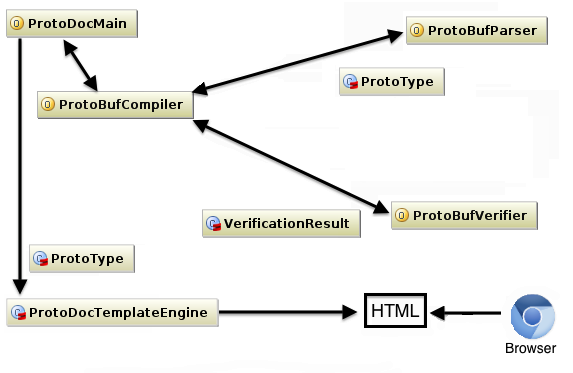
\includegraphics[scale=0.85]{main_classes.png}
\end{center}
\caption{Nieformalna wizualizacja interakcji pomiędzy komponentami}
\label{simple_visualization}
\end{figure}

Dzięki nie formalnej wizualizacji interakcji między komponentami na Rysunku \ref{simple_visualization} można łatwo zobrazować sobie
jak komponenty między sobą wymieniają informacje. Pliki *.proto są parsowane przez parser, po czym reszta komunikacji odbywa się na poziomie 
klas typu \verb|ProtoType|, oraz jej specjalizacji.

Jak widać mamy wydzielone klasyczne dla kompilatorów odpowiedzialności: parsowanie/skanowanie, weryfikację semantyczną oraz generowanie kodu.
W kolejnych sekcjach zostaną przedstawione diagramy oraz wizualizacje interakcji między tymi komponentami.

%------------------------------------------------------------------------------
\section{Architektura aplikacji}
\label{sec:sequence_diagrams}

W tej sekcji przedstawione zostaną diagramy sekwencji opisujące interakcje między wcześniej już wstępnie opisanymi komponentami.



Na diagramie sekwencji \ref{fig:sequence_diagram_parsing} zostało przedstawione szczegółowo do jakich interakcji między wcześniej opisywanymi (nie formalnie)
komponentami dochodzi podczas procesu parsowania. 

\begin{figure}[ch]
\begin{center}
 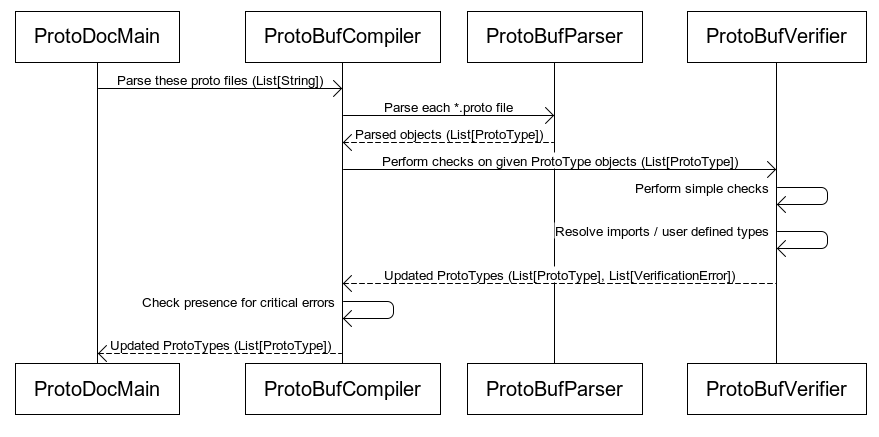
\includegraphics[width=\textwidth]{compile_sequence}
\end{center}
\caption{Diagram sekwencji parsowania oraz weryfikowania wiadomości}
\label{fig:sequence_diagram_parsing}
\end{figure}

Punktem wejściowym aplikacji jest klasa \verb|ProtoDocMain|, po sparsowaniu argumentów wejściowych specjalnym Domain Specific Language (innym niż
Parser Combinators, zostanie on omówiony i przedstawiony w sekcji poświęconej tej klasie), przekazuje przygotowane do parsowania zawartości plików
do obiektu \verb|ProtoBufCompiler|. Compiler jedynie deleguje parsowanie każdego z plików do \verb|ProtoBufParser|, który wykonuje parsowanie przy pomocy
\textit{Scala Parser Combinators}. 

Ponieważ jeden plik *.proto może zawierać więcej niż jedną wiadomość (lub enumerację), dla każdego sparsowanego
pliku proto zwracana jest lista typów konkretnych \textit{(omówionych szczegółowo w sekcji \ref{the_types})}, dziedziczących po abstrakcyjnej klasie \verb|ProtoType|. 

Kolejnym krokiem jest przekazanie otrzymanych właśnie \verb|ProtoType| do Instancji \verb|ProtoBufVerifier|, który zajmuje się weryfikacją poprawności typów.
Może on, ponieważ otrzymuje \textit{wszystkie} sparsowane typy, również rozstrzygnąć czy \textit{import} z innego pakietu jest poprawny czy też nie. 
Innymi słowy, jedną z jego odpowiedzialności jest rozwiązanie problemów widoczności typów. Nie mógł, oraz nie powinien, przeprowadzać tego Parser, ponieważ 
nie posiadał jeszcze pełnego zestawu danych (typów) koniecznych do rezolucji typów. Sposób w jaki informacja o ,,nie rozstrzygniętym typie'' jest przekazywana
do weryfikatora, jest dość prosty: Parser podczas napotkania typu którego jeszcze nie zna, tworzy taki sam obiekt referencji do pola, jaki stworzyłby gdyby
znał ten typ, jednak dodatkowo zaznacza iż typ nie był widoczny podczas parsowania. Gdy weryfikator dostaje wszystkie typy oraz ich pola, przeszukuje pola,
zważywszy na wspomnianą flagę - oraz próbuje dokonać rezolucji typu, mając już pełne informacje o dostępnych typach w danym kontekście. Przyjęta przez niego 
strategia zostanie przybliżona dokładniej w sekcji \ref{sec:verifier}.

\verb|ProtoBufVerifier| odpowiada listą komunikatów mogących być albo błędami, albo ostrzeżeniami, a \verb|ProtoBufCompiler| może na nie zareagować przerwaniem
wykonania aplikacji oraz wypisaniem wszystkich problemów, lub może zwrócić wszystkie zweryfikowane typy (obiekty typu \verb|ProtoType|) do głównej klasy programu,
która pierwotnie rozpoczęła proces parsowania plików proto --- do \verb|ProtoDocMain|.

Kolejnym krokiem w kierunku wytworzenia wyniku działania aplikacji --- gotowej strony www dokumentacji ProtoDoc --- jest 
przekazanie zweryfikowanych obiektów \verb|ProtoType| z \verb|ProtoDocMain| do ostatniego z istotnych komponentów aplikacji --- do generatora kodu, tj. 
do instancji klasy \verb|ProtoTemplateEngine|. Warty zauważenia jest powrót to nazewnictwa \textit{Proto\textbf{Doc}...} tej klasy, w przeciwieństwie do \textit{Proto\textbf{Buf}...}
występującego jako prefix poprzednich komponentów. Przyczyną takiego rozróżnienia w nazewnictwie jest, iż zarówno parser jak i weryfikator, nie są ściśle związane
z ProtoDoc - mogą parsować oraz weryfikować dowolne pliki proto, oraz zwracają ich obiektową reprezentację. Równie dobrze komponenty te można by wykorzystać
w innych celach - nie tylko celem generowania dokumentacji. 

Proces generowania kodu jest bardzo prosty. Jako, że \verb|ProtoBufCompiler| dostarczył już ,,gotowe'' obiekty, które na pewno są poprawne, jedyne co pozostaje
generatorowi do zrobienia to wygenerowanie strony HTML na podstawie każdego z obiektów proto-typów, które zostały mu przekazane przez \verb|ProtoDocMain|.

Diagramie sekwencji \ref{fig:generate_html_seq} obrazuje proces generowania kodu. Pierwsze dwie wymiany wiadomości zostały szczegółowo 
przedstawione na poprzednim diagramie (\ref{fig:sequence_diagram_parsing}).

\begin{figure}[ch]
\begin{center}
 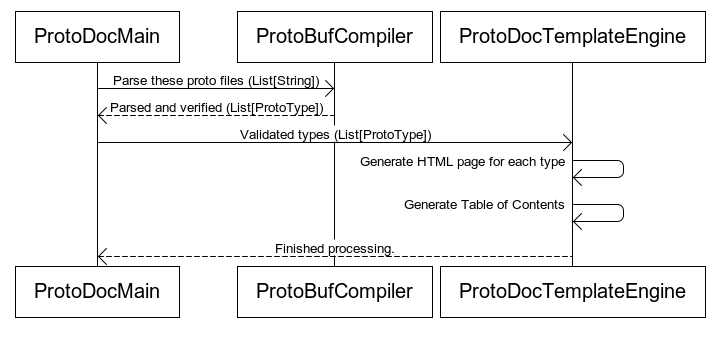
\includegraphics[scale=0.75]{generate_html_seq}
\end{center}
\caption{Diagram sekwencji generowania stron HTML dokumentacji}
\label{fig:generate_html_seq}
\end{figure}


%------------------------------------------------------------------------------
\subsection{Zastosowany model typów wiadomości Protocol Buffers w Scala}
\label{the_types}
Celem wykorzystania w pełni z potencjału statycznego typowania języka Scala --- zamiast pracowania wprost na listach i mapach wartości które 
w domyślnym przypadku zostałyby zwrócone przez parser, konieczne było stworzenie modelu typów, odzwierciedlającego w Scali typy mogące pojawić się w ProtoBuf.
Konieczne było zamodelowanie zarówno istniejącej wewnętrznie w Protocol Buffers jak i łatwej do rozszerzania o typy definiowanie przez użytkownika struktury typów.

Zdefiniowanie nowego typu przez użytkownika jest główną czynnością podczas opisywania interfejsu przy pomocy Google Protocol Buffers, także typy te powinny
również mieć istotne odzwierciedlenie w ProtoDoc. W ramach przypomnienia, Listing \ref{lst:super_simple_enum_and_message} przedstawia składnię zdefiniowania prostej 
wiadomości (\verb|message|) lub enumeracje (\verb|enum|) - jedynych interesujących nas w zakresie ProtoDoc typów. 

\begin{lstlisting}[caption={Przykład zdefiniowania nowych typów w Protocol Buffers IDL}, label={lst:super_simple_enum_and_message}]
package pl.project13;

/** some comments */
message MyNewType { required string pole = 1; }

/** some comments */
enum MyEnumeration { VALUE = 1; }
\end{lstlisting}

Okazuje się, że enumeracja i wiadomość dzielą wiele wspólnych cech, oba typy:
\begin{itemize}
 \item mogą znajdywać się w \textit{package},
 \item mają nazwę,
 \item mają ,,w pełni kwalifikowaną nazwę'', składającą się z połączenia nazwy typu,
 \item zawierają pola. Mimo, że w przypadku enumeracji pole wygląda nieco inaczej, można przyjąć pewne uogólnienie i traktować je tak samo jak pozostałe pola.
\end{itemize}

W związku zauważeniem powyższych wspólnych cech został wprowadzony wprowadzony typ \verb|ProtoType|, będący super-typem dla obu tych klass.

Dodatkowo warto zauważyć, że komentarze mogą być umieszczone \textit{,,na''} każdym z wspomnianych typów,
oraz to samo można powiedzieć o polach umieszczonych wewnątrz tych typów - jak obrazuje to Listing \ref{lst:comment_on_field}.

\begin{lstlisting}[caption = {Przykład umieszczenia komentarza ProtoDoc na polach wiadomości oraz enumeracji}, label = {lst:comment_on_field}]
message MyNewType { /** docs */ required string field = 1; }

enum MyNewType { /** docs */ SOME_VALUE = 1; }
\end{lstlisting}

Umieszczenie pola \textit{comment} wewnątrz klasy \verb|ProtoType| nie byłoby zatem dobrym pomysłem, ze względu na nie-możliwość ponownego użycia 
interfejsu typu ,,\textit{X} ma komentarz'' na polach. Rozwiązaniem jest wprowadzenie interfejsu ,,\verb|Commentable|'', które eksponuje metody związane
z posiadaniem komentarza, na przykład ,,czy komentarz jest obecny?'' etc. Pozwoliło to na implementację metod pracujących na tym interfejsie, 
nie ważne czy ów komentowalny element jest polem czy nowym typem, zatem zmniejszyło ścisłość wiązań w API tworzonego systemu. 

\begin{center}
\begin{tabular}{|p{\textwidth}|}
\hline
\hline
W przypadku języka Scala, mowa tutaj nie o interfejsach a \textit{Trait}ach (rozpoznawalnych na załączonych diagramach po zielonej ikonie \textbf{T}), 
jednak jako że celem tego rozdziału pracy nie przedstawienie implementacji a generalnego design projektu można przyjąć że Trait może być rozumiany
jako ,,interfejs''. Szczegółowy opis czym są \textit{Trait}y oraz jak wpływają na design projektu, można przeczytać w Sekcji \ref{sec:traits}, w Dodatku \ref{cha:appendixB}.
\\ \hline
\end{tabular}
\end{center}

\begin{figure}[ch]
\begin{center}
 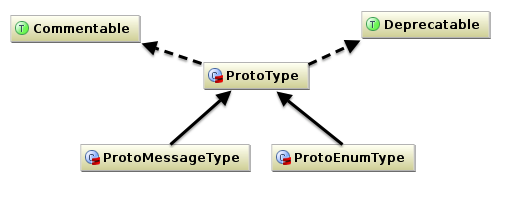
\includegraphics[width=\textwidth]{proto_types}
\end{center}
\caption{Zastosowany model typów definiowanlnych przez użytkownika typów}
\label{fig:types_diagram}
\end{figure}

Rysunek \ref{fig:types_diagram} przedstawia zastosowaną w projekcie strukturę typów. Warto zauważyć dodatkowy Trait o nazwie \verb|Deprecatable|, 
oznaczający ,,coś co może zostać adnotowane jako przestarzałe''. Adnotowanie pól jako \verb|@deprecated| jest dobrą praktyką programistyczną oraz 
bezcennym źródłem dodatkowej informacji o typie dla takiego narzędzia jak ProtoDoc, które może takie pola wyszarzyć lub zasugerować jakiego typu 
powinno się użyć zamiast oznaczonego taką adnotacją. Przyczyną wprowadzenia tego typu jako Trait ponownie jest fakt, że wiele elementów protocol buffers
może zostać oznaczona jako przestarzała, nie jedynie same deklaracje typów.

%------------------------------------------------------------------------------
\subsection{Zastosowany model typów pól Protocol Buffers w Scala}
\label{the_field_types}
Analogiczny jak przedstawiony powyżej problem dotyczy pól, które mogą być reprezentować jeden z predefiniowanych typów protocol buffers, lub
mogą być enumeracją lub wiadomością definiowaną przez użytkownika.

Celem skorzystania również i tutaj z statycznego typowania również podczas pracy na polach, również tutaj konieczne było wprowadzenie modelu typów.
Tutaj wymaganiem ponownie było aby możliwie prosto dało się wspierać już wbudowane w ProtoBuf jak i nowo definiowane przez użytkownika typy.

Listing \ref{lst:enum_and_msg_fields_dec} przedstawia różne możliwości jakie mamy do dyspozycji podczas definiowania pola w wiadomości lub enumeracji.
W przypadku gdy czytelnik chciałby się zagłębić w szczegóły składni oraz znaczenia poszczególnych deklaracji, zachęcam do przeczytania Dodatku \ref{cha:appendixA},
w którym wszystkie te elementy są szczegółowo omawiane. Przykład tutaj przytaczany jest celem unaocznienia ponownie cech wspólnych dla wspomnianych elementów.

\begin{lstlisting}[caption={Deklaracja pola w wiadomości oraz enumeracji}, label={lst:enum_and_msg_fields_dec}]
// message fields:
optional int32 age = 1;
required string age = 2 [default = "Konrad"];
repeated sint64 numbers = 3;

optional MyType it = 4;
optional MyEnum other = 5 [default = VALUE];

message MyType { }
enum MyEnum {
  // enum values:
  VALUE = 3;
}
\end{lstlisting}

Deklarowanie pól w wiadomościach jest oczywiście bardziej interesujące niż pola w enumeracjach, co powyższy przykład powinien dość ładnie obrazować.
Mimo wszystko, ponownie jesteśmy w stanie znaleźć pewne wspólne elementy pomiędzy wszelkimi ,,polami'', włączając w to również wartości enumeracji.
Przy okazji, pamiętajmy iż każde  z tych pól może być \textit{Deprecated} oraz może zostać okomentowane komentarzem ProtoDoc.

\begin{itemize}
 \item pole posiada nazwę,
 \item pole posiada przypisany mu \textit{tag} (liczba umieszczona po znaku równości, po szczegółowe wyjaśnienie czym tag jest, odsyłam do Dodatku \ref{cha:appendixA}),
 \item pole może posiadać komentarz,
 \item pole może być ozaczone jako przestarzałe (\textit{Deprecated}).
\end{itemize}

Powyższa lista elementów wspólnych w sposób oczywisty doprowadziła do powstania klasy \verb|ProtoField| będącej podstawą ku wszystkim pozostałym typom.
Dzięki wydzieleniu Traitów \verb|Commentable| oraz \verb|Deprecatable|, również teraz można je zastosować aby osiądnąć te same funkcjonalności w nowo przedstawionych klasach.

Pole będące wartością enumeracji będziemy traktować analogicznie jak zwyczajny \verb|ProtoField|, nie jest ono wyjątkowe z perspektywy struktury samej z siebie.
Co je odróżnia od \verb|ProtoMessageField| jest natomiast fakt iż po \verb|ProtoMessageField| dziedziczą wszystkie predefiniowane typy.
Dokładne oddanie relacji pomiędzy utworzonymi tutaj typami a typami umieszczanymi w plikach proto nie jest w naszym przypadku konieczne, a być może nawet nie wskazane.
W przypadku korzystania z protocol buffers na platformie JVM, nie istnieją odpowiedniki typów unsigned / signed - także korzystamy w tym przypadku po prostu z 
typu \verb|scala.Int|, do przechowania np. \textit{wartości domyślnej} takiego pola. Nazwa typu którego dana klasa jest mapowaniem zostaje jednak utrzymana w ciele klasy,
abyśmy mogli podczas generowania dokumentacji przywołać jaki dane pole miało typ w pliku *.proto. Pełen spis przyjętych mapowań został przedstawiony w formie Tabeli \ref{tab:field_types}. 

\begin{figure}[ch]
\begin{center}
 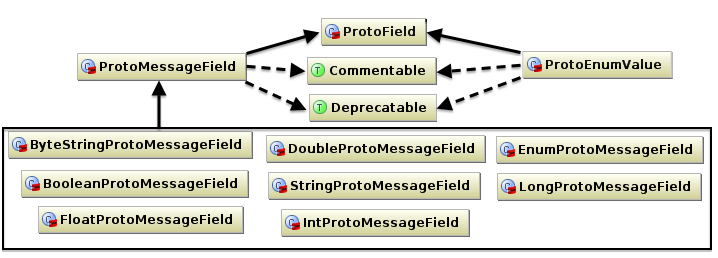
\includegraphics[width=\textwidth]{fields_types}
\end{center}
\caption{Zastosowany model typów pól mogących wystąpić w ProtoBuf IDL}
\label{types_diagram}
\end{figure}

W ramach ciekawostki, chciałbym w tym miejscu przedstawić implementację dwóch przykładowych z omawianych klas.

\begin{lstlisting}[caption={Pełna implementacja klasy ProtoEnumValue}, label={lst:protoenumvalue}]
case class ProtoEnumValue(valueName: String, tag: ProtoTag)
  extends ProtoField
  with Commentable
  with Deprecatable
\end{lstlisting}

\begin{lstlisting}[caption={Pełna implementacja klasy StringProtoMessageField}, label={lst:stringprotomessagefield}]
case class StringProtoMessageField(override val fieldName: String,
                                   override val tag: ProtoTag,
                                   override val modifier: ProtoModifier,
                                   override val defaultValue: String = None)
  extends ProtoMessageField(fieldName, 
                            "string", // type name in *.proto
                            "java.lang.String", // JVM representation
                            tag, 
                            modifier,
                            defaultValue)
\end{lstlisting}

Warto zwrócić uwagę, że mimo iż klasy przedstawiona na Listingach \ref{lst:protoenumvalue} oraz \ref{lst:stringprotomessagefield} nie posiadają stricte 
zdefiniowanego ciała, dzięki pewnym konwencjom oraz mechanizmom udostępniamym przez Scala, takie definicja są 
wszystkim co jest potrzebne do zdefiniowania w pełni funkcjonalnych klas, włącznie z polami, akcesorami dla atrybutów etc.

Czytelnika zainteresowanego mechanizmami kryjącymi się za zastosowanymi tutaj ,,\verb|case class|ami'' zachęcam do przeczytania sekcji \ref{sec:caseclass},
dotyczącej tego działu języka Scala, z Dodatku \ref{cha:appendixB}.

\begin{table}
 \begin{center}
\begin{tabular}[c]{|c|c|}
\hline 
Typ pola w Protocol Buffers & Odpowiednik w ProtoDoc\\ \hline

double   & DoubleProtoMessageField \\ \hline
float    & FloatProtoMessageField \\ \hline
int32    & IntProtoMessageField \\ \hline
int64    & LongProtoMessageField \\ \hline 
uint32   & IntProtoMessageField \\ \hline 
uint64   & LongProtoMessageField \\ \hline 
sint32   & IntProtoMessageField \\ \hline 
sint64   & LongProtoMessageField \\ \hline 
fixed32  & IntProtoMessageField \\ \hline 
fixed64  & LongProtoMessageField \\ \hline 
sfixed32 & IntProtoMessageField \\ \hline 
sfixed64 & LongProtoMessageField \\ \hline 
bool     & BooleanProtoMessageField \\ \hline
string   & StringProtoMessageField \\ \hline 
bytes    & ByteStringProtoMessageField \\ \hline \hline 
enumeration type & EnumProtoMessageField(type) \\ \hline
user defined message type & ProtoMessageField(type) \\ \hline \hline 
enum value & ProtoEnumValue \\ \hline
 \end{tabular}
 \end{center}
\caption{Typy pól oraz odpowiadające im typy Scala \small{(bazując na reprezentacji typów przez protoc na JVM)}}
\label{tab:field_types}
\end{table}


%===========================================================================
\chapter{Szczegóły implementacyjne}
\label{sec:zastosowanePodejscie}

Poniższy rozdział przedstawi szczegóły implementacyjne poszczególnych komponentów składających się na \textit{ProtoDoc}.
Ogólna architektura oraz interakcie między komponentami zostały już opisane w poprzednim rozdziale, stąd te kwestie nie bądą tutaj ponownie poruszane,
uwaga natomiast zostanie skoncentrowana na szczegółach implementacyjnych, oraz ewentualnych wyjaśnieniach nowo wprowadzanych pojęć lub bibliotek.

Omówione zostaną zarówno ogólne założenia przyjęte podczas projektowania systemu, jak i struktura klas przyjęta celem
modelowania struktury typów Protocol Buffers. Następnie przedstawione zostaną poszczególne komponenty aplikacji, z naciskiem na uzasadnienie
wybranych rozwiązań oraz rozważenia ich zalet, wad oraz potencjalnych możliwości usunięcia zauważonych wad. 

Na zakończenie rozdziału przedstawione zostaną elementy kodów źródłowych, skrócone do postaci wystarczającej na cel omówienia danego tematu 
- w przypadku chęci zapoznania się ze całością implementacji np. komponentu parsera, zachęcam do zapoznania się 
z załączonymi do pracy plikami źródłowymi projektu.

\begin{center}
\begin{tabular}{ | p{\textwidth} | }
\hline 
Jako że poniższy rozdział wymaga od czytelnika minimalnej choćby znajomości Scala oraz Protocol Buffers IDL, zalecane jest zapoznanie się z 
dodatkami \ref{cha:appendixA} (Protocol Buffers) oraz \ref{cha:appendixB} (Podstawy języka Scala). \\ \hline
\end{tabular}
\end{center}


%---------------------------------------------------------------------------
\section{ProtoBufParser}
\label{sec:protoBufParser}
Parser został zaimplementowany przy pomoy wspominanych wielokrotnie już kombinatorów parserów, 
dostarczanych wraz z biblioteką standardową Scali. Jako wiadomość referencyjną, służącą jako przykład parsowanego pliku *.proto, 
będziemy posługiwać się w tym rozdziale bardzo prostą wiadomością, obejmującą jednak podstawowe funckojalności definiowania typów
w Protocol Buffers, przedstawioną na Listingu \ref{lst:my_sample_simple_message}.

\newpage 
\begin{lstlisting}[caption={Przykład wiadomości, służący łatwiejszej wizualizacji działania parsera}, label={lst:my_sample_simple_message}]
message MyMessage {
  required FullName name = 1;
  optional int32 age = 2 [default = 1];
  optional Gener gender = 3;

  message FullName {
    required string firstname = 1;
    required string lastname = 2;
  }

  enum Gender {
    MALE = 1;
    FEMALE = 2;
  }
}
\end{lstlisting}

Parser jest zdefiniowany jako obiekt dziedziczący po klasie \verb|RegexParsers| (patrz Listing \ref{lst:define_the_parser_object}), będącą domyślną implementacją
dostarczającą metody \verb|parse| oraz \verb|parseAll|, konieczne do implementacji parsera. Ponad wspomniane funkcje,
udostępnia również możliwość ignorowania białych znaków oraz kilka metod pomocniczych. Wszystkie najważniejsze metody 
zawarte są w Traicie \verb|Parsers|, którego RegexParsers dostaje wmieszanego (jak wytłumaczono w Dodatku \ref{cha:appendixB}).

\begin{lstlisting}[caption={Definicja obiektu parsera}, label={lst:define_the_parser_object}]
object ProtoBufParser
  extends RegexParsers // includes the parser DSL
  with ImplicitConversions // conversions for list flattening
  with ParserConversions // my implicic conversions
  with Logger { // include a logger
\end{lstlisting}

Dodatkowo wmieszane zostały dwa Traity udostępniające implicit konwersje (patrz Dodatek \ref{cha:appendixB}, Sekcja \ref{sec:implicit} -- Implicit Conversions),
ułatwiające pracę z listami oraz konwertowanie między typami takimi jak proste typy liczbowe do typu reprezentującego tag protobufowy (klasa \verb|ProtoTag|).

Idąc dalej przyjrzymy się najprostrzemu parserowi w tej klasie. Będzie to proste wyrażenie regularne matchujące identyfikatory które można stosować w 
plikach *.proto. Intentyfikatory te mają podobne warunki istnienia jak indentyfikatory w Java, także wyrażenie (de facto, cały ,,parser indentyfikatora'') 
tak jak to przedstawiono na Listingu \ref{lst:simplest_parser_possible_23}

\begin{lstlisting}[caption={Bardzo prosty parser, zdefiniowany za pomocą implicita, który rozszerza API klasy String o metodę \textit{r} tworzącą wyrażenie regularne (instancję klasy \textit{scala.util.matching.Regex})},label={lst:simplest_parser_possible_23}]
val ID = """[a-zA-Z_]([a-zA-Z0-9_]*|_[a-zA-Z0-9]*)*""".r
\end{lstlisting}

Następnie zdefiniujemy mały parser wykorzystując powyższy (Listing \ref{lst:messageTypeName}):

\begin{lstlisting}[caption={Definicja parsera identyfikatora wiadomości}, label={lst:messageTypeName}]
def messageTypeName /*: Parser[String]*/ = "message" ~> ID
\end{lstlisting}

Znak \verb|~>| oznacza \textit{kombinację parserów, przy odrzuceniu lewej strony}. W efekcie zdefiniowaliśmy właśnie część gramatyki
oznaczającą iż jeżeli pojawi się słowo message, powinien po nim nastąpić pewien identyfikator, ale dla celów obróbki tej informacji, będzie nas interesować tylko
parser po prawej stronie znaku \verb|~>|. Lewa strona zostanie jedynie użyta podczas parsowania, oraz słowo ,,message'' nie będzie widoczne podczas dalszego
kombinowania tego parsera z pozostałymi.

\begin{center}
\begin{tabular}{|p{\textwidth}|}
\hline Warto zauważyć iż znak \verb|~| jak i jego odpowiedniki ,,porzucające'' lewą (\verb|~>|) lub prawą (\verb|<~|) stronę sekwencji 
parserów, po pierwsze: nie są operatorami, a metodami, oraz po drugie: są dostarczane przez implicit konwersje na parserach lub typach prostych. 
 (Szczegółowy opis znajduje się w Dodatku \ref{cha:appendixB}).\\
\hline
\end{tabular}
\end{center}

Kolejnym potrzebnym do zdefiniowania parserem jest właściwe ciało wiadomości. Definicja jest bardzo prosta i czytelna, ponieważ korzystamy tutaj z 
zdefiniowanych gdzie indziej parserów poszczególnych pól. Listing \ref{lst:parsowanie_pola_znaczy_ciala} przedstawia parser ciała wiadomości,
który niebawem zostanie użyty wspólnie z parserem nazwy wiadomości celem budowy pełnego obiektu wiadomości przy pomocy kombinacji tych parserów.

W ramach przypomnienia zanim spojrzymy na kod parsera ciała wiadomości przypomnijmy sobie jakie elementy może ono zawierać:
\begin{itemize}
 \item definicję pola wiadomości,
 \item definicję zagnieżdżonej wiadomości,
 \item definicję zagnieżdżonej enumeracji.
\end{itemize}

Powyższe trzy typy mogących wystąpić w ciele wiadomości deklaracji bardzo łatwo jest przetłumaczyć na parser,
przedstawiony na Listingu \ref{lst:parsowanie_pola_znaczy_ciala}.


\begin{lstlisting}[caption={Parser ciała wiadomości}, label={lst:parsowanie_pola_znaczy_ciala}]
def messageBody = "{" ~> 
                        rep(instanceField | enumTypeDef | messageTypeDef) 
                    <~ "}"
\end{lstlisting}

Listing \ref{lst:parsowanie_pola_znaczy_ciala} poza znanym nam już kombinatorem \verb|~>| wykorzystuje jeszcze kombinator \verb|rep()|,
oznaczający po prostu iż dany element może powtarzać się wielokrotnie. Jego działanie jest analogiczne do znaku \verb|+| w wyrażeniach regularnych.

Poza parserem ciała wiadomości umieszczonym na Listingu \ref{lst:parsowanie_pola_znaczy_ciala}, konieczne oczywiście jest zdefiniowanie parserów \verb|enumTypeDef|,
\verb|messageTypeDef| oraz \verb|instanceField|. Implementacje tych parserów, są stosunkowo długie także nie zostaną umieszczone w calości w tym dokumencie. Jako
przykład zostanie podane jednak pierwsze kilka linii metody definicji, pozwalającej nam zapznać się z generalną zasadą działania wszystkich zaimplementowanych w 
projekcie parserów, ich kombinacji oraz jak dochodzi to przekształcenia zwyczajnego drzewa syntaktycznego do zaprojektowanych przez nas w porzednim rozdziale klas.

\begin{lstlisting}[caption={Skrócona implementacja parsera pola wiadomości}, label={lst:short_field_parser}]
def instanceField = opt(comment) ~ modifier ~! (protoType | userDefinedType) ~ ID ~! "=" ~! integerValue ~ opt(defaultValue) <~ ";" ^^ {
    case doc ~ mod ~ pType ~ id ~ eq ~ tag ~ defaultVal =>
      val comment = doc.getOrElse("") // : Option[String]
      // ...

      // return the prepared instance
      if(isResolvedType) {
        if(isKnownProtoEnumField(pType))
          // ... 
          ProtoMessageField.toEnumField(id, itsEnumType, tag, mod, defaultVal)
        else 
          // ...
          ProtoMessageField.toProtoField(pType, id, tag, mod, defaultVal)
      } else {
        // ...
        ProtoMessageField.toUnresolvedField(pType, id, tag, mod, defaultVal)
      }
}
\end{lstlisting}

Z nowych elementów pojawiły się tutaj metody \verb/|/ (działającej analogicznie do logicznej alternatywy) oraz \verb|^^| będącej operacją transformacji 
przeparsowanego ciągu. Operacja \verb|^^| jest jedną z najistotniejszych ponieważ pozwala zmianę produkcji parsera z 
zwyczajnych list, do faktycznych obiektów, które zamodelowaliśmy w poprzednim rozdziale. Szczegóły składni jej wykonania są dość złożone, jednak w skrócie, 
mamy tutaj do czynienia z funkcją wyższego rzędu, której przekazujemy funkcję która będzie w stanie transformować sparsowany ciąg, do typu ProtoType.
W naszym przykładzie zwracany jest \verb|ProtoMessageField| z pobranych podczas parsowania elementów. Słowo kluczore \verb|return| znane z innych języków programowania
nie jest tutaj konieczne.

Pozostałe parsery są bardzo podobne w implementacji do przedstawionych powyżej, oraz generalnie sprowadzają się głównie do sprawdzania poprawności,
na przykład wartości domyślnej w przypadku znanego przez parser już typu oraz przypisań odpowiednich elementów do odpowiednich typów, które szczegółowo omówiono w poprzednim rozdziale.

~\\\*

% \subsection{Wprowadzenie do kombinatorów parserów}
% TODO klasyfikacja, opisać że są lewostronnie rekurencyjne etc.
% 
% \verb|http://en.wikipedia.org/wiki/Recursive_descent_parser|
% 
% \verb|http://en.wikipedia.org/wiki/Left_recursion|
% \verb|http://en.wikipedia.org/wiki/Parser_combinator|
% 
% \verb|http://stackoverflow.com/questions/17840/how-can-i-learn-about-parser-combinators|


%---------------------------------------------------------------------------
\section{ProtoBufVerifier}
\label{sec:verifier}
Klasa \verb|ProtoBufVerifier| pojawiła się z konieczności przeprowadzania rozwiązania typów (ang. \textit{rype resolution}),
w przypadku gdy mamy do czynienia z odwołaniem się do typu zdefiniowanego albo ,,poniżej'' typu zawierającego to odwołanie,
lub na przykład w innym pliku. Parser niestety nie jest wówczas w stanie rozstrzygnąć samodzielnie czy dany typ, na przykład zastosowany na polu wewnąrz wiadomości,
jest nie zdefiniowany czy po prostu został zdefiniowany w innym miejscu, do którego parser jeszcze nie doszedł. Verifier unika tych problemów, pracę po zakończeniu 
działania parsera, kiedy to wszystkie informacje o typach są już dostępne.

Przechodząc do klasy \verb|ProtoBufVerifier|, mamy już zakończony parsing oraz przekazane wszystkie sparsowane typy do instancji tej klasy.
\verb|ProtoBufVerifier|, podobnie jak Parser, również jest zdefiniowany jako \textbf{object}, co odrobinę upraszcza korzystanie z niego.
Patrząc na Verifier z zewnątrz (z poziomu \verb|ProtoDocCompiler|a) użycie go sprowadza się do wykonania weryfikacji na komplecie 
przygotowanych przez parser obiektów ProtoType, oraz następnie sprawdzenie czy zawierają błędy ,,krytyczne''. 
Fragment kodu odpowiedzialny za te czynności, umieszczony w \verb|ProtoDocCompiler| został przedstawiony na listingu \ref{lst:verify_how_it_is_called}

\begin{lstlisting}[caption={Przykład wykorzystania weryfikatora}, label={lst:verify_how_it_is_called}]
val verification= ProtoBufVerifier.verify(parsedProtos)

if(verification.invalid) {
  verification.errors.foreach(error(_)) // print all errors
  throw new ProtoDocVerificationException(verification)
}
\end{lstlisting}


Implementacja weryfikatora bazuje głównie na zebranych informacjach oraz pojęciu ,,kontekstu'' (na przykład ,,wewnątrz tej wiadomości'')
dzięki któremu jest w stanie rozstrzygnąć czy widoczność typów jest poprawna etc. Zaimplementowane weryfikacje różnią się dla typów wiadomości 
oraz enumeracji. Poszczególne weryfikacje zostaną opisane w kolejnej sekcji. Listing \ref{lst:verify_this_please} przedstawia na jakiej zasadzie
Weryfikator deleguje wykonanie sprawdzeń poprawności do konkretnych wyspecjalizowanych metod.

\begin{lstlisting}[caption={Delegacja sprawdzania poprawności typów},label={lst:verify_this_please}]
def verify(protoTypes: List[ProtoType]): VerificationResult = 
  VerificationResult((for (protoType <- protoTypes) 
                       yield check(protoType, protoTypes)).flatten)
\end{lstlisting}

~

\begin{lstlisting}
def check[T <: ProtoType](protoType: T, 
                          protoTypes: List[T]): List[VerificationError] = 
  protoType match {
    case msgType: ProtoMessageType =>
      checkMessageType(msgType, protoTypes)
    case enumType: ProtoEnumType =>
      checkEnumType(enumType, protoTypes)
}
\end{lstlisting}

Tutaj zastosowanie znajduje \textbf{pattern matching}, znany z języków funkcyjnych, takich jak \textit{Haskell} lub \textit{Erlang}.
Konstrukcja \textbf{match} pozwala na dekonstrukcję matchowanego typu oraz wiele bardzo potężnych operacji które w przeciwnym przypadku 
byłyby bardzo długą serią instrukcji warunkowych oraz rzutowań typów. Metoda \verb|check| jak widać, deleguje wiadomość jeszcze głębiej, 
jednak tym razem już do specjalizowanych metod odpowiadających za sprawdzanie poprawności typu. Przykładem implementacji checków jest 
\verb|checkMessageType| umieszczony na listingu \ref{lst:checkMessageType}.

\begin{lstlisting}[caption={Metoda checkMessageType, sprawdzająca poprawność wiadomości}, label={lst:checkMessageType}]
def checkMessageType(msgType: ProtoMessageType, protoTypes: List[ProtoType]) = {
  info("Running verifications on "+b(msgType)+" message")

  // errors 
  val tagErrors = TagVerifier.validateTags(msgType, msgType.fields.map(_.tag))

  val enumErrors = for (enum <- msgType.enums) yield checkEnumType(enum, protoTypes)
  val fieldErrors = for (field <- msgType.fields) yield checkField(msgType, field, protoTypes)
  val innerMsgErrors = for (innerMsg <- msgType.innerMessages) yield checkInnerMsg(msgType, innerMsg, protoTypes)

  // warnings 
  val deprecatedItemsCount = checkDeepDeprecation(msgType)
  warn("Found "+deprecatedItemsCount+" deprecated fields/types in ["+msgType.fullName+"]")

  tagErrors ::: fieldErrors.flatten ::: enumErrors.flatten ::: innerMsgErrors.flatten ::: Nil // return a list of all errors
}
\end{lstlisting}


\subsection{Obsługiwane weryfikacje}
\textit{ProtoDoc} w momencie pisania tej pracy obsługuje następujące weryfikacje poprawności (dla wszystkich typów pól oraz deklaracji typów jakie parser obecnie 
jest w stanie zrozumieć):

\begin{itemize}
 \item poprawność \textbf{tag}ów: 
  \subitem czy tag zawiera się w specyfikowanym przez Protocol Buffers zakresie dozwolonych liczb, 
  \subitem czy tag jest niepowtarzalny w zasięgu bloku danej wiadomości lub enumeracji.
 \item czy typ definiowany przez użytkownika posiada niepowtarzalną w pełni kwalifikowaną nazwę, 
 \item czy wartość domyślna pola w wiadomości posiada typ zgodny z typem tego pola (np. liczbę całkowitą dla pól int32), 
 \item czy w przypadku korzystania z definiowanego przez użytkownika typu, wykorzystanego podczas deklaracji pola, typ ten jest ,,widoczny'' 
       z wewnąrz kontekstu tego pola, 
 \item czy wiadomość lub enumeracja nie posiada zduplikowanych nazw pól.
\end{itemize}

Najciekawszą z wspomnianych weryfikacji jest definitywnie sprawdzanie widoczności typu, z racji wielu możliwości odwołania się do niego,
na przykład podczas deklaracji pola w wiadomości. Całość implementacji jest b. długa, jednak celem zobrazowania jak można budować czytelne weryfikacje
przy pomocy pisania własnych implicit conversions, zostaną przytoczone w Listingu \ref{lst:visibilityChecks} najciekawsze fragmenty metody odpowiedzialnej
za sprawdzenie czy typ danego pola jest ,,w zasięgu''.

\begin{lstlisting}[caption={Ważniejsze fragmenty implementacji sprawdzania widoczności typu}, label={lst:visibilityChecks}]
  // by using the find method on List
  val fullyQualifiedMatch = allParsed.find(_.fullName == typeName)
  if(fullyQualifiedMatch.isDefined) {
    field resolveTypeTo(fullyQualifiedMatch.get)      
    return NoErrorsEncountered
  } 
    
  //by using an infix notation, via implicit conversions
  if(typeName isDefinedWithin fromContext) {
    val resolvedType = typeName getResolvedTypeWithin fromContext
    field resolveTypeTo(resolvedType)      
    return NoErrorsEncountered
  }
  // ... 
  // unable to resolve, report error
  error("the field: ["+field.fieldName+"] was unresolvable at this point...")
  return UndefinedTypeVerificationError(field.fieldName, "Unable to resolve type ["+typeName+"] from ["+fromContext+"] context.") :: Nil
\end{lstlisting}


Dodatkowo zostały zaimplementowane ostrzeżenia, które nie są błędne w kontekście Protocol Buffers,
jednak są ,,podejrzane'' stąd warto wskazać je programiście podczas poszukiwania problemów w kodzie:

\begin{itemize}
 \item czy enumeracja nie jest pusta (nie posiada żadnych wartości),
 \item czy wiadomość nie jest pusta (nie posiada żadnych pól).
\end{itemize}

Weryfikacje te były bardzo proste w implementacji dzięki zaprojektowanemu modelowi danych. Jako przykład może posłużyć sprawdzenie czy typ jest pusty, 
przedstawione w całości w Listingu \ref{lst:checkIfEmpty}.

\begin{lstlisting}[caption={Implementacja ostrzeżenia czy enumeracja jest pusta}, label={lst:checkIfEmpty}]
def checkIfEmpty(enumType: ProtoEnumType) {
  if(enumType.values.isEmpty)
    warn("""|The enum "+enumType.fullName+" has no values.
            |This could be a possible typo with missplacing the "}"..."""
            .stripMargin)
}
\end{lstlisting}

Weryfikacje są bardzo ciekawym elementem ProtoDoc, oraz jednym z najbardziej obiecujących miejsc do dalszego rozwoju.
Nie trudno jest sobie wyobrazić wiele heurystycznych metod mogących tutaj znaleźć zastosowanie, oraz pomóc programiście
pracować nad poprawianiem jakości tworzonych przez siebie wiadomości. Tymczasem, podstawowe checki, które zostały
zaimplenentowane w tym projekcie powinny być wystarczające - zważywszy na fakt iż są dodatkiem, a nie właściwym celem aplikacji.

%---------------------------------------------------------------------------
\section{ProtoDocTemplateEngine - generator kodu}
Ostatim komponentem składającym się na ProtoDoc jest generator kodu, w naszym przypadku jego rolę pełni klasa \verb|ProtoDocTemplateEngine|.

Jego rola jest bardzo prosta, jecyne co musi zrobić to dla każdego otrzymanego typu, wygenerować stronę HTML, z przygotowanego wcześniej szablonu.
Dodatkowym krokiem jest wygenerowanie strony z indeksem wszystkich typów, aby użytkownik mógł wygodnie wyszukiwać.

Strony generowane są przy wykorzystaniu biblioteki \textit{Scalate} \cite{Scalate}
oraz silnika \textbf{Mustache} dostarczanego przez nią. Mustache jest prostym językiem definiowania szablonowym (ang. \textit{template}), który umieszcza 
się np. w HTMLu. Silnik mustache następnie jest w stanie iterować np. po dostarczonej mu liście pól danej wiadomomości oraz wyświetlać fragment szablonu dla każgego z nich.

Na tym kończy się odpowiedzialność \verb|ProtoDocTemplateEngine| --- proste zmapowanie pól obiektów, na odpowiadające im nazwy w szablonach.
Przykład przekazania informacji o typie dla strony o typie enumeracji można zobaczyć na Listingu \ref{lst:using_scalate}. Metoda \verb|engine.layout|
zwraca wygenerowaną stronę jako String, pozostaje jedynie ją zapisać na dysk.

\newpage
\begin{lstlisting}[caption={Przykład zastosowania Scalate (z silnikiem renderowania szablonów Mustache)}, label={lst:using_scalate}]
def renderEnumPage(enum: ProtoEnumType) = {
  import enum._

  val data = Map("enumName" -> typeName,
    "packageName" -> packageName,
    "comment" -> comment,
    "values" -> values)

  engine.layout("enum".mustache, data)
}
\end{lstlisting}

\subsection{Język szablonów - Mustache}
\label{sec:mustache}
Celem krótkiego przedstawienia języka Mustache \cite{Mustache}, oraz uzasadnienia wybrania takiego silnika renderującego szablony chciałbym przedstawić kilka elementów Mustache.
Posłużymy się jedynie kilkuliniowymi przykładami, aby nie zaciemniać obrazu HTMLem który aż tak interesujący z naszej perspektywy nie jest.

Nazwa silnika \textit{Mustache} pochodzi od angielskiego słowa oznaczającego wąsy. Może się to wydawać dziwne, lecz po pierwszym spojrzeniu na 
znaczniki mustache etymologia nazwy staje się oczywista: Wszystkie odwołania do zmiennych, jak i operacje warunkowe obejmowane są 
następującym znakiem: \verb|{{  }}|, przypominającym wąsy. Konkretny przykład zastosowania umieszczania zmiennych w HTML można zobaczyć na Listingu \ref{lst:simpleMustache}.

\begin{lstlisting}[label={lst:simpleMustache}]
<title>ProtoDoc for: {{packageName}}.{{fieldName}}</title>
\end{lstlisting}

Warunki natomiast zapisuje się przy pomocy znaku rozpoczynającego warunek: \verb|{{#boolean_var}}| (lub jego odpowiednikowi negującemy wartość w sprawdzanej zmiennej:
\verb|{{^boolean_var}}|) oraz kończącego blok warunkowy \verb|{{/boolean_var}}|. 
Identyczną składnią (\verb|{{#fields}}|) można iterować po wartościach zawartych w liście, co w ProtoDoc ma miejsce podczas np. renderowania
tabeli z informacjami wszystkich pól danego typu.

Mustache udostępnia odrobinę więcej funkcjonalności niż omówione powyżej, jednak w przypadku generowania prostych szablonów, 
z jakimi mamy do czynienia w ProtoDoc, nie były one konieczne do zastosowania.


%---------------------------------------------------------------------------
% \chapter{Przygotowanie środowiska do rozwoju ProtoDoc}
% \label{sec:prepare_env}
% W rozdziale ten pokrótce przedstawię jak należy przygotować środowisko programistyczne celem rozwijania narzędzia \textit{ProtoDoc},
% może się to okazać przydatne w przypadku chęci sprawdzenia testów jednostkowych bądź wprowadzenia nowych funkcjonalności do aplikacji.
% 
% \section{Instalacja narzędzia SBT}
% ProtoDoc budowany oraz testowany jest przy wykorzystaniu najpopularniejszego obecnie narzędzia do zarządzania buildem w świecie programistów Scala:
% Simple Build Tool, w śkrócie zwanym SBT \footnote{SBT - Strona domowa projektu: \href{https://github.com/harrah/xsbt}{https://github.com/harrah/xsbt}}.


%===========================================================================
\chapter{Przykład zastosowania ProtoDoc w realnym projekcie}
\label{maven}

W poniższym rozdziale zostanie przedstawione zastosowanie narzędzia ProtoDoc, w parze z Apache Maven \cite{Maven}, obecnym
de facto standardem zarządzania dużymi projektami w świecie aplikacji klasy enterprise.

W tym celu został zaimplementowany dodatkowy ,,\textit{plugin}'' (ang. wtyczka) do Maven, pozwalający na automatyczne 
wykonanie ProtoDoc podczas procesu budowy projektu. Zostanie również przedstawiony sposób w jaki ten plugin można skonfigurować,
z poziomu pliku konfiguracyjnego Mavena.

\section{Przykład połączenia ProtoDoc z Maven, celem automatycznego generowania dokumentacji}
Ponieważ takie narzędzie jak \textit{ProtoDoc} powinno być stosowane w sposób w pełni automatyczny, logicznym krokiem w rozpowszechnieniu
jego użycia była integracja z najpopularniejszym (de facto ,,standardowym'') narzędziem zarządzania cyklem życia projektu, jakim w świecie Javy jest \textbf{Maven}.

W związku z powyższym w ramach projektu został zrealizowany plugin do narzędzia Maven. Wspierane są zarówno wersje 2.x jak i 3.x tego narzędzia. 
Nie będziemy tutaj wnikać w szczegóły i zasady działania narzędzia Maven, ponieważ jest to bardzo obszerny temat, jednak
przedstawię jak można wykorzystać \textit{ProtoDoc} wraz z Mavenem do automatycznego generowania dokumentacji wszystkich plików proto umieszczonych w projekcie.

Wszystkie zależności jak i pluginy deklaruje się w mavenie w pliku \textbf{pom.xml}. W naszym przypadku konieczne będzie dodanie elementu \verb|<plugin>|, wewnątrz
\verb|project -> build -> plugins|.

\begin{lstlisting}[caption={Deklaracja korzystania z pluginu ProtoDoc}, label={last:use_the_maven_plugin}]
      <plugin>
	<groupId>pl.project13.maven</groupId>
	<artifactId>protodoc-maven-plugin</artifactId>
	<version>1.0</version>
	<executions>
	  <execution>
	    <goals>
	      <goal>package</goal>
	    </goals>
	  </execution>
\end{lstlisting}
\begin{lstlisting}[caption={Kontunuacja listingu \ref{last:use_the_maven_plugin}}]
	</executions>
  <!-- Optional overrides of default properties:
	<configuration>
	  <protoDir>${project.basedir}/src/main/proto</protoDir>
	  <outDir>${project.basedir}/target/protodoc</outDir>
	  <verbose>false</verbose>
	</configuration>  -->
      </plugin>
\end{lstlisting}

Jest to wystarczające aby ProtoDoc mógł \textbf{automatycznie}, podczas budowania projektu generować dokumentację
dla wszystkich plików proto umieszczonych wewnątrz domyślnego folderu - \textbf{src/main/proto}. Ścieżka ta jest zgodna z konwencjami przyjętymi
w Maven, jednak w razie potrzeby istnieje możliwość nadpisania tego ustawienia poprzed dodanie elementu configuration, tak jak to przedstawiono na Listingu \ref{last:use_the_maven_plugin}.

%------------------------------------------------------------------------------
\section{Szczegóły implementacyjne}
\label{maven_implementacja}
Uważny czytelnik zauważył że przeniknęliśmy właśnie ze świata \textbf{Scala} do świata \textbf{Javy}.
Wartym podkreślenia jest jak sprawnie da się korzystać z obu tych języków ,,jednocześnie'', 
dzięki dobrodziejstwom platformy JVM \footnote{JVM - Java Virtual Machine} --- wspólnego runtime na którym różne języki bezproblemowo mogą 
się między sobą komunikować.

Dzięki poprzednim doświadczeniom w tworzeniu pluginów mavenowych, oraz przygotowaniu ProtoDoc w taki sposób aby był bardzo łatwo używalny nie tylko z poziomu
command line, ale również poziomu kodu źródłowego, integracja z mavenem przebiegła bardzo prosto. Pliku pom.xml zawierającego zależności pluginu nie będę 
tutaj umieszczał z racji jego rozmiaru (~150 linii), jednak okazuje się że cała implementacja pluginu, bezproblemowo nadaje się to umieszczenia w tym miejscu.

\begin{lstlisting}[caption={Pełna implementacja pluginu mavenowego korzystającego z ProtoDoc}]
public class ProtoDocMojo extends AbstractMojo {
  /** @parameter default-value="${project.basedir}/src/main/proto" */
  private String protoDir;
  /** @parameter default-value="${project.basedir}/target/protodoc" */
  private String outDir;
  /** @parameter default-value="false" */
  private boolean verbose;

  public void execute() throws MojoExecutionException {
    ProtoDocMain.generateProtoDoc(protoDir, outDir, verbose);
  }
}
\end{lstlisting}

Ciekawostką jest że pierwotne wersje Maven2, były tak stare, iż nie były jeszcze dostępne adnotacje w Javie. 
Stąd uciekano się do \textit{meta-programowania} w komentarzach, poprzez tak zwane docklety --- adnotacje (słowa poprzedzane znakiem \verb|@|)
umieszczone nad zmiennymi prywatnymi powyższego Mojo faktycznie \textbf{są znaczące} oraz deklarują iż w te zmienne powinny zostać wstrzyknięte
przez mavena odpowiednie ustawienia z sekcji \verb|<configuration/>| pluginu.

%------------------------------------------------------------------------------
\section{Efekt działania ProtoDoc wraz z Maven}
Efektem zastosowania powyższego pluginu w projekcie mavenowym, jest automatyczne wygenerowanie się dokumentacji.
Aby unaocznić bardziej strukturę plików oraz proces korzystania z Apache Maven \cite{Maven}, poniżej przedstawiam krótką sekwencję komend
wydaną w zgognej z POSIX linii poleceń, obrazującej działanie mavena oraz samego pluginu.

\begin{verbatim}
$ tree
+-- pom.xml
+-- src
    +-- main
        +-- java
        |  +-- pl
        |      +-- project13
        |          +-- ProtoDocMojo.java
        +-- proto
            +-- amazing_message.proto
            +-- common_message.proto
            +-- simple.proto
$ mvn clean install
# ............. maven output .............
$ tree
+-- pom.xml
+-- src/ ...
+-- target
    +-- clases/ ...
    +-- protodoc
    |   +-- images/ ...
    |   +-- js/ ...
    |   +-- index.html 
    |   +-- pl.project13.AmazingMessage.EnumType.html
    |   +-- pl.project13.CommonMessage.html
    |   +-- pl.project13.MessageWithInner.html
    |   +-- pl.project13.MessageWithInner.InnerMessage.html
\end{verbatim}

Powyższy listing ładnie obrazuje jaką strukturę katalogów generuje ProtoDoc w efekcie działania.
Folder \verb|target| jest w projektach mavenowych dedykowany wszystkim produktom danego procesu budowania projektu.
ProtoDoc umieszcza swoje pliki analogicznie jak uczyniłby to JavaDoc plugin (generujący dokumentację dla kodu zapisanego w języku Java),
wewnątrz folderu \verb|target/| z własnym sub katalogiem o nazwie \verb|protodoc|.

Aby zobaczyć jak wygenerowana dokumentacja wyląda na żywo, można uruchomić na przykład poniższą komendę, uruchamiającą przeglądarkę Google Chromium:

\begin{lstlisting}
$ chromium-browser target/index.html
\end{lstlisting}

Przykładowe zrzuty ekranu z działającej aplikacji przedstawione zostały w na następnej stronie, w seksji \ref{sec:screenshots}.

%---------------------------------------------------------------------------
\newpage
\section{Zrzuty ekranu wygenerowanej dokumentacji}
\label{sec:screenshots}
W tej sekcji zostały umieszczone zrzuty ekranu z przykładowych wygenerowanych stron dla różnych typów wiadomości.

\begin{figure}[hc]
 \begin{center}
  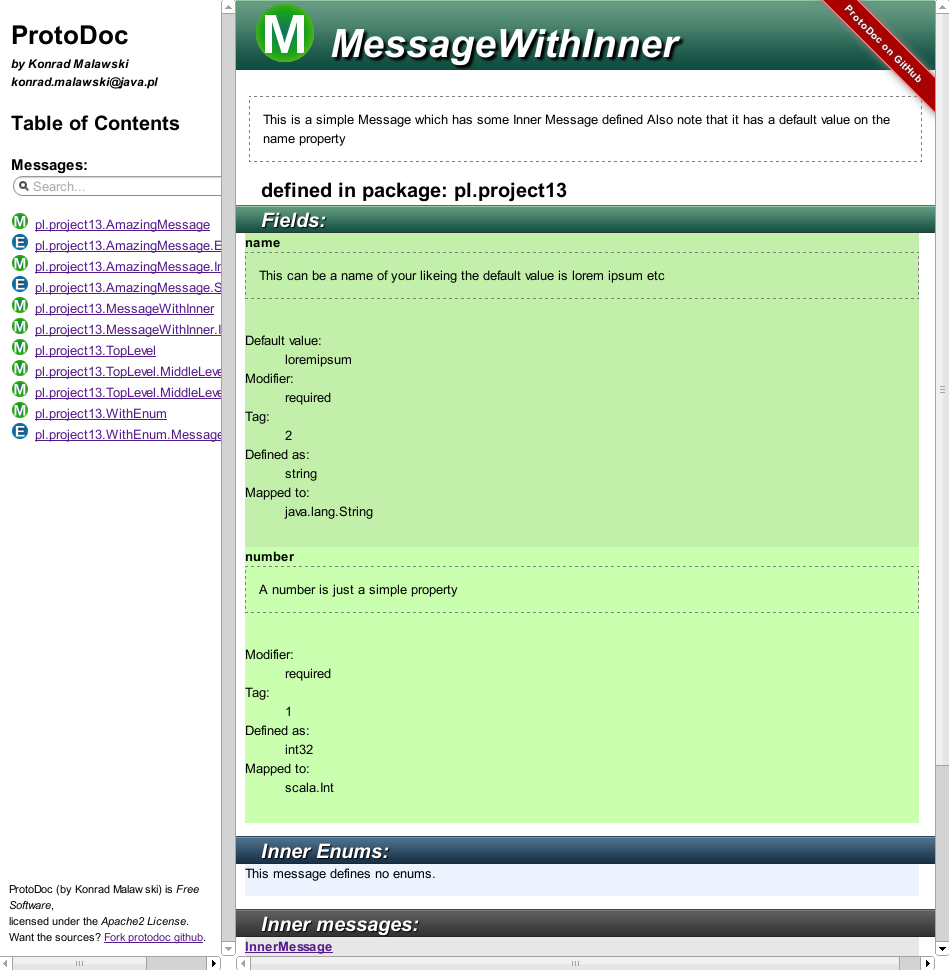
\includegraphics[scale=0.5]{../protodoc_main.png}
  % protodoc_main.png: 949x970 pixel, 93dpi, 25.92x26.50 cm, bb=0 0 735 751
 \end{center}
 \caption{Widok wygenerowanej strony dla typu \textbf{message}}
 \label{msg_page}
\end{figure}

Na Rysunku \ref{msg_page} przedstawiona została strona wygenerowana na podstawie prostej wiadomości.
Widok wiadomości składa się na jego nazwę, wyróżnioną jako nagłówek strony, dokumentację umieszoną na jego typie,
informacji o pakiecie w którym została ona zdefiniowana oraz liście pól oraz wewnętrznych enumeracji oraz wiadomości zdefiniowanych w niej.
Każde z pól dokumentowane jest swoją nazwą, odpowiednim typem na platformie JVM (co w przypadku typów definiowanych przez użytkownika może być praktyczne),
oraz oczywiście właściwą dokumentacją umieszczoną na danym polu.

Widoczna jest również po lewej stronie lista wszystkich wiadomości oraz enumeracji przeparsowanych podczas generowania dokumentacji
dla tego projektu. Dodatkowo możliwe jest wyszukiwanie po wspomnianych elementach poprzez umieszone nad nimi pole temu służące.
Wyszukiwarka ta jest praktyczna ponieważ filtruje ona listę wiadomości po dowolnym podciągu znaków, dzięki czemu łatwo jest znaleźć
wszystkie wiadomości mające na przykład w nazwie ,,Person''.

\begin{figure}[hc]
 \begin{center}
  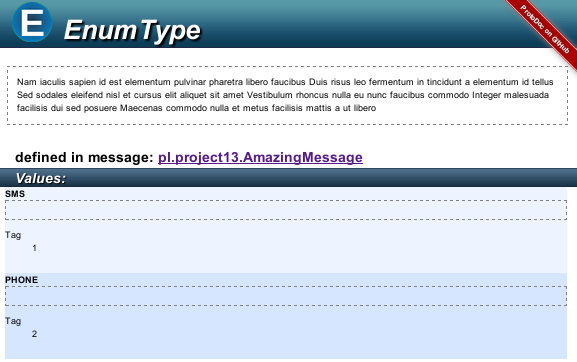
\includegraphics[width=\textwidth]{../protodoc_enum.png}
  % protodoc_enum.png: 949x970 pixel, 93dpi, 25.92x26.50 cm, bb=0 0 735 751
 \end{center}
 \caption{Widok wygenerowanej strony dla typu \textbf{enum}}
 \label{enum_page}
\end{figure}

Na Rysunku \ref{enum_page} przedstawiona jest strona enumeracji. Celem pokazania całej tej strony,
a nie ,,całości'' widoku jak miało to miejsce na Rysunku \ref{msg_page} została tutaj pominięta lewa ramka (spis typów).
Z racji, iż mamy do czynienia z enumeracją, kolor strony jest zmieniony oraz ikonka \textbf{M} została zmieniona na \textbf{E}.
Dalsze części strony są zbudowane analogicznie - wpierd dokumentaja umieszczona na typie enumeracji a następnie lista jej pól,
które w przypadku enumeracji należy rozumieć jako wartości. Każda wartość może mieć przypisaną dokumentację, umieszczoną w 
prostokącie poniżej jej nazwy, oraz wartość taga.

%---------------------------------------------------------------------------
\chapter{Rola testów w procesie tworzenia aplikacji}
\label{chapter:tdd}

Rozdział ten ma za cel przybliżyć czytelnikowi jak istotną rolę w rozwoju \textit{ProtoDoc} miały testy jednostkowe
(oraz w pewnym sensie również integracyjne). Dzięki zastosowaniu poniżej opisanej metodyki, możliwe było otrzymanie
kodu którego większość funckojalności jest pokryta testami a API jest na tyle stabilne, iż wprowadzanie zmian w jednym miejscu
nie ma znaczącego wpływu na pozostałe komponenty.

W pierwszej sekcji przedstawiona zostanie metodyka \textit{Test Driven Development}, w skrócie TDD,
oraz jak należy ją stosować.

W drugiej sekcji zostanie przedstawione wyjście jakie ujrzy się w momencie uruchomienia testów w ProtoDoc.
Zaskakujące może się wydać jak czytelne są wiadomości logowane przez framework testowy ScalaTest \cite{ScalaTest}.

\section{Metodyka TDD i jej pozytywny wpływ na projekt}

Projekt prowadzony był zgodnie z zasadami Test Drivem Development (zwanego dalej \textit{TDD}),
co znacznie ułatwiło ustabilizowanie API oraz głównych konceptów jeszcze we wczesnych etapach tworzenia aplikacji.
Ponad to, metodyka ta umożliwiła pracę z dotychczas nieznanym mi API bez obaw o zniszczenie zaimplementowanych wcześniej funkcjonalności.

Metodykę \textit{TDD} możnaby opisać jako cylk składający się z trzech faz:
\begin{itemize}
 \item napisanie najpierw \small{(sic!)} testu, sprawdzającego automatycznie czy stawiane przed nami oczekiwanie zostało spełnione
 \subitem pewną sub-fazą jest upewnienie się że test faktycznie na stan obecny aplikacji nie przechodzi. Najlepiej aby wiadomość niepowodzenia
          jasno wskazywała na to co jest przyczyną problemu. Jest to istotne nie tyle teraz, podczas implementacji, jednak podczas dalszego rozwoju aplikacji,
          kiedy to być może sprawimy, że warunek sprawdzany ten test przestanie być prawdziwy - wówczas, \textit{,,kilka tygodni później''}, pomocny komunikat o przyczynie problemu 
          znacznie przyśpieszy zlokalizowanie oraz naprawienie problemu.
 \item implementacji funkcjonalności, tak aby warunki w teście zostały spełnione.
  \subitem należy pamiętać aby była to implementacja minimalna - nie wolno wychodzić ,,do przodu'' z implementacją, nawet jeżeli uważa się,
           że pewna funkcjonalność \textit{prawdopodobnie} będzie niebawem implementowana.
 \item oraz refaktoringu właśnie zaimplementowanych komponentów aplikacji, lub zauważonych podczas implementacji ewentualnych powtórzeń kodu itp.
\end{itemize}

Fazy te w literaturze znane są jako ,,Red - Green - Refactor'', i obrazuje się ją przy pomocy przedstawionego na Rysunku \ref{tdd_cycle} grafu.

\begin{figure}[ch]
 \begin{center}
  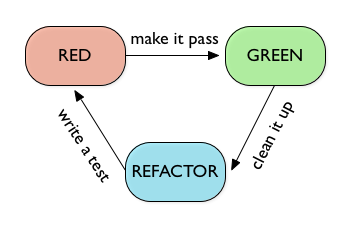
\includegraphics[scale=0.8]{tdd_cycle}
 \end{center}
 \caption{Schemat obrazujący fazy pracy w metodyce \textit{TDD} \small{(źródło: własne)}}
 \label{tdd_cycle}
\end{figure}


Przedstawiony powyżej cykl zazwyczaj trwa pomiędzy kilkoma a trzydziestoma minutami. Technika ta jest ściśle związana z samo-dyscypliną programisty
i stosunkowo trudna do zastosowania w przypadku nie stosowania jej na codzień - jednak rezultaty, pod postacią wzrostu jakości kodu oraz zmniejszeniu 
czasu traconego na poszukiwania błędów są znaczne.

Oprócz pisania testu zanim powstanie jakakolwiek implementacja, bardzo ważnym elementem fazy implementacji jest jest aby jej celem 
było napisanie \textit{minimalnej ilości kodu doprowadzając test to ,,przejścia''} (spełniania wymagań w nim stawianych). Przykładowo, nie dozwolone jest
implementowanie dodatkowych funkcjonalności (,,na zapas''), nawet jeżeli uważa się iż będą niebawem konieczne podczas fazy implementacji związanej 
z właśnie napisanym testem. Faza implementacji nie może zostać zakończona w przypadku uszkodzenia (sprawienia że inny niż obecnie rozwijany test ,,nie przejdzie'').

Dzięki zastosowaniu tej metodyki, nie dość że kod tworzyło się łatwiej -- dzięki skupianiu się na konkretnym celu, dostarczającym konkretnych wartości dla projektu -- 
ale również podczas wprowadzania dużych zmian, mogłem być pewien, że nie uszkadzam przypadkiem istniejących oraz działających sprawnie elementów programu.
Szczerze zalecam stosowanie tej metodyki, a nawet jeżeli nie czystego TDD, które może byż z początku przytłaczającym podejściem do wytwarzania oprogramowania,
to z pewnością do samego rozpoczyniania pracy od napisania testu, a dopiero następnie przestępowania do programowania.

Ogółem w projekcie zostało zaimplementowane ponad 46 testów, w których zastosowano ponad 200 asercji.

\section{Zaimplementowane specyfikacje}
Ponieważ wyjście z Runnera (,,tego który uruchamia'') testów stosowanego przezemnie w tym projekcie, są bardzo czytelne, oraz ładnie dokumentują 
jakie funkcjonalności dokładnie zostały zaimplementowane oraz automatycznie przetestowane. Poniżej umieszczone zostały jedynie niektóre z wiadomości,
ponieważ umieszczenie wszystkich zajęłoby niestety kilka stron -- mam jednak nadzieję, że ich czytelność mile zaskoczy czytelnika oraz zachęci do stosowania
tego typu podejścia do testowania aplikacji.

\begin{verbatim}
ProtoBufVerifierTest:
The Verifier should validate field types 
- should detect an unresolvable field
  + Given a message with an invalid fieldtype 
  + When the message is parsed and verified 
  + Then the Verifier report it as invalid 
  + And it should point out that the UnknownType is unresolvable 
- should have no problems with resolvable field Type
  + Given a message with valid, resolvable fieldtype, defined before the message 
  + When the message is parsed and verified 
  + Then the result should contain one HasResolvableField message 
  + And the field should be resolved to the propper type 

RealSimpleParsingTest:
Parsing of an real message, with outer enum 
- should be parsed properly
  + Given A real proto file 
  + When it is parsed 
  + And it is verified 
  + Then parsed size should be 2 
  + And the inner message should be detected 
  + And the inner message should be named properly 
  + And the enum field should have the proper type resolved 
  + And it's tag should be equal 3 
  + And it's resolved type should be the outer enumeration 
  + And the outer enum should be parsed and named properly 
...
\end{verbatim}

Jak widać, informacje drukowane podczas uruchamiania testów mogą wręcz stanowić swego rodzaju dokumentację jego zachowania.
Są czytelne oraz zachowują wspólną formę dzięki czemu łatwo jest znaleźć przy jakich warunkach początkowych, można oczekiwać 
jakiego rezultatu działania aplikacji.

%---------------------------------------------------------------------------
\chapter{Podsumowanie}
\label{cha:podsumowanie}
Celem powstania aplikacji ProtoDoc było udostępnienie programistom, pracującym z Google Protocol Buffers na codzień, narzędzia 
automatycznie dokumentującego tworzone przez nich wiadomości. Cel został osiągnięty poprzez implementację parsera 
oraz generatora kodu, działającego na zasadach podobnych do JavaDoc, znanego i popularnego narzędzia generującego dokumentację
dla klas zapisanych w języku Java. Przy okazji implementacji tych dwóch komponentów okazało się, że dodanie trzeciego - weryfikatora,
nie dość że byłoby bardzo proste, to również zwiększyłoby znacznie przydatność ProtoDoc. 

W finalnej wersji aplikacji, weryfikator został zaimplementowany oraz posiada kilka podstawowych weryfikacji, takich jak sprawdzanie poprawności
przypisanych wartości domyślnych, wartości tagów czy też raportowania napotkanych pól Deprecated (ang. ,,przestarzałych''). 
Weryfikacje stanowią największe potencjalne pole do rozwoju narzędzia, ponieważ można by zaimplementować liczne dodatkowe heurystyki 
sprawdzające poprawność tworzonej wiadomości pod kątem utrzymywalności w przyszłości.

Wszystkie funkcjonalności aplikacji, włączając w to parsowanie ,,nietypowych sytuacji'' oraz wszystkie weryfikacje, sprawdzane na różnych przypadkach
zostały pokryte testami automatycznymi. W momencie pisania projekt zawierał 49 testów, zawierających łącznie ponad 200 asercji, z których wszystkie podczas
uruchamiania testów są spełniane. Dzięki rygotystycznie stosowanej podczas implementacji tego projektu metodyce Test Driven Development, udało się utrzymać kod na 
wysokim poziomie czystości oraz komponeny nie posiadające dużych zależności, co dobrze świadczy o przyjętym projekcie systemu.
Kod oczywiście dzięki temu był i jest również prosty do testowania o czym świadczyć może wspomniana już duża liczba testów automatycznych, 
dających pewność, że zaimplementowane funkcjonalności faktycznie działają.

W ramach umożliwienia faktycznego stosowania ProtoDoc w rzeczywistości został również zaimplementowany plugin do systemu zarządzania cyklem życia projektu - 
Apache Maven \cite{Maven} - dzięki któremu dołączenie ProtoDoc do istniejących projektów jest bardzo proste -- ogranicza się do konfiguracji pluginu w pliku konfiguracyjnym docelowego projektu.
Wspomniany plugin został również dołączony do niniejszej pracy, jako jej naturalne rozszerzenie.

Podsumowując projekt zakończył się sukcesem -- wszystkie wymagania dotyczące generowania dokumentacji oraz automatyzacji tego procesu zostały spełnione.
Zakres projektu został nawet nieco poszerzony z racji dołączenia komponentu weryfikującego kod. Aplikacja posiada duży potencjał na dalszy rozwój
w kierunku stania się używanym ,,w rzeczywistości'' narzędziem, a punkty w których można by kontunuować ów rozwój zostały wymienione w kolejnej, ostatniej już, sekcji też pracy.

\section{Plany rozwoju aplikacji}
Aplikacja w przyszłości może zostać rozszerzona aby wspierać jeszcze większą część standardu 
Protocol Buffers, w szczególności, można wyróźnić niektóre interesujące zadania do wykonania:

\begin{itemize}
 \item zaimplementować rozpoznawanie słowa kluczowego \textbf{option}, służącego przekazywaniu pewnych meta danych do kompilatora \textit{protoc},
 \item zaimplementować bardziej dokładne rozwiązywanie widoczności, biorące pod uwagę różne notacje z kropką w nazwie wiadomości
       w przypadku stosowania słowa kluczowego \textit{import},
 \item dobudować dodatkowy moduł, który dokumentowałby elementy \textbf{service}, które nie zostały pokryte w tej pracy,
 \item zaimplementować więcej, oraz bardziej wnikliwych weryfikacji, służących nie tylko jako sprawdzenie poprawności, ale jako rady oraz utrzymanie dobrego stylu
       implementowanych wiadomości,
 \item zaimplementować \textit{ProtoDoc} jako plugin do innych systemów zarządzania cyklem życia projektu. Zadanie to jest stosunkowo proste, 
       jak już przedstawiono na przykładzie Maven, a mogłoby znacznie pomóc społeczności użytkowników języków takich jak Groovy bądź Scala, gdzie Maven 
       jest rzadziej wykorzystywany niż w projektach ,,czysto Javowych''.
\end{itemize}

Projekt planuję rozwijać w czasie wolnym, ponieważ uważam że potrzeba takiego narzędzia faktycznie istnieje oraz przy okazji jego 
implementacji nauczyłem się wiele o Scali jak i samych Protocol Buffers.


%---------------------------------------------------------------------------
\appendix
\chapter{Podstawy języka Scala}
\label{cha:appendixA}
Celem tego dodatku jest przybliżenie czytelnikowi języka ,,Scala'' aby w wystarczająco płynny sposób mógł czytać przykłady kodu używane w tym dokumencie.

%---------------------------------------------------------------------------
\section{Krótka historia języka}
\label{sec:scala_history}
Język Scala (,,Scalable Language'') najłatwiej jest przedstawić jako hybrydę dwóch znanych nurtów programowania: programowania obiektowego oraz funkcyjnego, wraz z 
powiązanymi z nimi językami programowania. Twórca języka Scala, Martin Oderski\cite{odersky_scala}

Jako konkretnych ,,rodziców'' można by wskazać: 
\begin{itemize}
 \item \textbf{Java} - jako reprezentant nurtu obiektowego 
 \item oraz języki: \textbf{Haskell}, \textbf{SML} oraz pewne elementy języka \textbf{Erlang} (głównie \textit{Actor model}).
\end{itemize}


%---------------------------------------------------------------------------
\section{Podstawy}
\label{sec:scala_basics}
Ta sekcja służy przybliżeniu czyletnikowi języka \textit{Scala} na poziomie wystatczającym aby swobodnie czytać przykłady
kodu umieszczone w tej pracy. W niektórych przykładach pomijane są przypadki skrajne lub nietypowe, celem szybkiego oraz 
jasnego przedstawienia minimum wiedzy na temat języka aby móc swobodnie go ,,czytać''.

\textit{Scala} jest językiem statycznie typowanym posiadającym lokalne ,,Type Inferrence''. Pozwala to kompilatorowi 
\textit{scalac} na ,,odnajdywanie'' typów wszystkich zmiennych oraz typów zwracanych przez metody podczas kompilacji,
bez potrzeby definiowania ich wprost. System ten

Użycie nawiasów \verb|()|, średnika \verb|;| oraz kropki \verb|.| jest analogiczne jak w przypadku Javy, 
jednak w wielu przypadkach opcjonalne gdyż kompilator jest w stanie wydedukować gdzie powinny się znaleźć.
\begin{lstlisting}
 val value = Option(42);
 val other = value.orElse(0);

 // moze zostac zastąpione
 val value = Option(42)
 val other = value orElse 0
\end{lstlisting}

Jednym z ciekawych przykładów stosowania notacji bez nawiasów i kropek jest \textit{ScalaTest}\footnote{ScalaTest - framework do testowania - http://www.scalatest.org}
(przy którego pomocy pisano testy w tym projekcie). Przykładowa \textit{asercja} napisana w \textit{DSL}u definiowanym przez tą bibliotekę wygląda następująco:
\begin{lstlisting}
 messages should (contain key ("Has") and not contain value ("NoSuchMsg"))
\end{lstlisting}



%---------------------------------------------------------------------------
\section{Scala Parser Combinators}
\label{sec:scala_parser_combinators}

\chapter{Podstawy języka Scala oraz Scala Parser Combinators}
\label{cha:appendixB}
Celem tego dodatku jest przybliżenie czytelnikowi języka ,,Scala'' aby w wystarczająco płynny sposób mógł czytać przykłady kodu używane w tym dokumencie.

%---------------------------------------------------------------------------
\section{Krótka historia języka}
\label{sec:scala_history}
Język Scala (,,Scalable Language'') najłatwiej jest przedstawić jako hybrydę dwóch znanych nurtów programowania: programowania obiektowego oraz funkcyjnego, wraz z 
powiązanymi z nimi językami programowania. Twórca języka Scala, Martin Oderski \footnote{Martin Odersky - Strona domowa: \href{http://lamp.epfl.ch/~odersky/}{http://lamp.epfl.ch/~odersky/}}
był ściśle związany z językiem Java - był głównym projektantem generyków w Javie (\textit{Java Generics}) oraz głównym autorem utrzymywanej po dziś dzień
serii kompilatorów \textbf{javac} \footnote{Wywiad z Martinem Odersky na temat korzeni języka Scala - \href{http://www.artima.com/scalazine/articles/origins_of_scala.html}{www.artima.com/.../origins\_of\_scala}}.

Jako konkretnych ,,rodziców'' można by wskazać: 
\begin{itemize}
 \item \textbf{Java} - jako reprezentant nurtu obiektowego 
 \item oraz języki: \textbf{Haskell}, \textbf{SML} oraz pewne elementy języka \textbf{Erlang} (głównie \textit{Actor model}).
\end{itemize}


%---------------------------------------------------------------------------
\section{Podstawy}
\label{sec:scala_basics}
Ta sekcja służy przybliżeniu czyletnikowi języka \textit{Scala} na poziomie wystatczającym aby swobodnie czytać przykłady
kodu umieszczone w tej pracy. W niektórych przykładach pomijane są przypadki skrajne lub nietypowe, celem szybkiego oraz 
jasnego przedstawienia minimum wiedzy na temat języka aby móc swobodnie go ,,czytać''.

\textit{Scala} jest językiem statycznie typowanym posiadającym lokalne ,,Type Inferrence''. Pozwala to kompilatorowi 
\textit{scalac} na ,,odnajdywanie'' typów wszystkich zmiennych oraz typów zwracanych przez metody podczas kompilacji,
bez potrzeby definiowania ich wprost. System ten

Użycie nawiasów \verb|()|, średnika \verb|;| oraz kropki \verb|.| jest analogiczne jak w przypadku Javy, 
jednak w wielu przypadkach opcjonalne gdyż kompilator jest w stanie wydedukować gdzie powinny się znaleźć.
\begin{lstlisting}
 val value = Option(42);
 val other = value.orElse(0);

 // moze zostac zastąpione
 val value = Option(42)
 val other = value orElse 0
\end{lstlisting}

Jednym z ciekawych przykładów stosowania notacji bez nawiasów i kropek jest \textit{ScalaTest}\footnote{ScalaTest - framework do testowania - http://www.scalatest.org}
(przy którego pomocy pisano testy w tym projekcie). Przykładowa \textit{asercja} napisana w \textit{DSL}u definiowanym przez tą bibliotekę wygląda następująco:
\begin{lstlisting}
 messages should (contain key ("Has") and not contain value ("NoSuchMsg"))
\end{lstlisting}

Dostępne jest wiele sposobów definiowania metod / pól w klasie,
w efekcie (na poziomie bytecode), wszystkie przekładane są na wywołania metod. Dostępne są słowa kluczowe:
\begin{itemize}
 \item \textbf{def}, \textit{def}iniujący zwyczajną metodę instancyjną. Warto nadmienić że Javowa koncepcja pojęcia \textit{static} nie jest dostępna z poziomu Scala.
 \item \textbf{val}, deklarujący ,,stałą'' - to jest metodę która raz zawołana, zwróci wartość oraz pole to będzie konsekwentnie zwracać tą samą wartość. 
              Dodatkowym efektem jest traktowanie zmiennych tego typu analogicznie do Javowych zmiennych z modyfikatorem \textbf{final}.
 \item \textbf{var}, deklaruje zwyczajną ,,zmienną'', do jakiej przyzwyczajeni jesteśmy z Java.
 \item modyfikator \textbf{lazy}, wpływający na moment inicjalizacji zmiennej - metody zadeklarowane z modyfikatorem \textbf{lazy} 
       zostaną dopiero zainicjalizowane podczas pierwszego odwołania się do tego pola z innego miejsca w kodzie. 
       W przypadku pary \textbf{lazy val}, metoda ta zostanie zawołana jedynie jednokrotnie, a zwrócona po raz pierwszy wartość
       zostanie zapisana w cache oraz będzie konsekwentnie zwracana podczas ponownych wywołań tej metody.
\end{itemize}

Modyfikator lazy pozwala na eleganckie budowy konstrukcji stosowanych w Parser Combinators, omówionych poniżej.


%---------------------------------------------------------------------------
\section{Traits - wmieszanie zachowania do klasy}
\label{sec:traits}

Słowo kluczowe \textbf{trait} rozpoczyna definicję typu zwanego traitem.
Implementacja nie różni się (na potrzeby tego szybkiego omówienia) od implementowania klasy,
jednak różnica jest podczas ,,dziedziczenia'' przy wykorzystaniu traitów. Nie mówimy bowiem o ,,dziedziczeniu'' 
w przypadku \textit{trait}ów, a o ,,wmieszaniu'' (ang. \textit{mixin} - wmieszanie) zachowania do klasy konkretnej.

Poniżej został przedstawiony najprostrzy trait zawierający jakieś zachowanie, oraz jeden ze sposobów jego wmieszania do klasy konkretnej.
Warto zauważyć że w przypadku wmieszania \textit{trait}a \verb|A| do klasy \verb|Test|, wprowadzamy między nimi relację ,,Test \textbf{IS-A} A'',
analogicznie jak w przypadku dziedziczenia.

\begin{lstlisting}
trait A { 
  def test = "A" // definicja metody zwracającej "A"
}

class Test extends A { } // wmieszanie A

new Test().test // skompiluje i wykona sie poprawnie
\end{lstlisting}

Co ciekawe, nie zauważamy różnicy w przypadku składni odnoszącej się do dziedziczenia dwóch klas konkretnych, oraz wmieszania traita.
Składnia ulega zmianie w przypadku korzystania z więcej niż jeden trait lub domieszania traita do klasy która już dziedziczy po innej klasie,
wówczas zamiast słowa kluczowego \textbf{extends} należy stosować \textbf{with} (nie dozwolone jest wielokrotne zapisanie \textbf{extends},
jednak wielokrotne \textbf{with} są często spotykane). Przykład wmieszania większej ilości traitów zostanie przedstawiony poniżej.

Jest to namiastka dziedziczenia wielobazowego jednak Scala dzięki swojemu bardzo rygorystycznemu kompilatorowi jest w stanie 
uniknąć sytuacji gdzie dziedziczenie wielobazowe byłoby niebezpieczne (klasyczne przykłady 
problematycznych sytuacji w przypadku dziedziczenia wielobazowago można przeczytać w ,,Symfonii C++'', autorstwa pana Grębosza \cite{symfonia}).

Kompilator \textit{scalac} przy napotkaniu konflintów nazw mogących doprowadzić do niejasności ,,którą metodę należy zawołać'', nie skompiluje takiego kodu
oraz poprosi o rozwiązanie konfliktu w sposób explicite. Jako przykład rozważmy dwa \textit{trait}y udostępniające metodę \verb|def test: String|:

\begin{lstlisting}
trait A { def test = "A" }
trait B { def test = "B" }

class Example extends A with B {
  // blad kompilacji!
}
\end{lstlisting}

Przy napotkaniu problemu tego typu kompilator zgłosi:
\begin{verbatim}
error: overriding method test in trait A of type => java.lang.String;
                  method test in trait B of type => java.lang.String needs `override' modifier
class Example extends A with B {
\end{verbatim}

Dzieje się tak ponieważ \textbf{scalac} próbuje odnaleźć która metoda powinna mieć większą wagę, a tymsamym powinna zostać wywołana.
Ponieważ nie jesteśmy w stanie dodać modyfikatora \textbf{override} do żadnego z \textit{trait}ów (ponieważ nie nadpisują one tej metody, a jedynie deklarują),
jedynym możliwym miejscem na rozwiązanie tego konfliktu jest uzupełnienie \verb|Example| o następujący fragment kodu, rutujący poprawnie nasze wywołanie metody:

\begin{lstlisting}
class Example extends A with B {
 // selektywne odwolanie sie do metody konkretnego supertypu
 override def test = super[B].test
}

new Example().test // poprawne
\end{lstlisting}




%---------------------------------------------------------------------------
\section{Scala Parser Combinators}
\label{sec:scala_parser_combinators}


%---------------------------------------------------------------------------
\bibliographystyle{alpha}
\bibliography{myrefs}

\end{document}
